%PART_1_CHAP_1
\myChapter{L}{a robotique}
%WAIT a Review ok
\begin{resumChap}
Ce premier chapitre a pour objet de présenter les différentes contraintes aujourd'hui liées au monde de la robotique.\par%
Dans un premier temps, nous verrons quelles sont les possibilités légales d'utilisation, de réutilisation et de dérivation du matériel robotique.
Nous verrons comment certaines de ces contraintes influent sur le développement de projet et les conséquences implicites de celles-ci. Notamment, nous caractériserons les communautés issues de projet open source.\par%
Dans un second temps, nous présenterons différents éléments spécifiques à la robotique et plus particulièrement à la robotique éducative. Ainsi, nous évoquerons des caractéristiques générales telles que la mobilité ou la forme des robots, ou encore les types de programmation (visuelle ou textuelle) associés. Enfin, nous donnerons plusieurs exemples de robots aujourd'hui développés pour un usage éducatif.
\end{resumChap}
\section{La robotique open source}
    \subsection{La philosophie de l'open source}\label{sec:open}
        \paragraph{Fondement et origine}
            La notion d'open source s'est notamment développée en parallèle de la capacité à dupliquer (à l'identique) un contenu et ainsi de le redistribuer à son propre intérêt. Aujourd'hui, il est vu comme un préalable nécessaire à une utilisation plus créative, riche et collaborative des contenus en facilitant leur diffusion et leur dérivation. Mais, elle s'est d'abord construite par opposition au brevet et au copyright en offrant des alternatives plus ouvertes. 
            \myPhantom{subparagraph}{Brevet}
                Un brevet est un titre de propriété industrielle qui confère à son titulaire un monopole d'exploitation sur l'invention brevetée pour une durée maximale de 20 ans. Les premières traces de ce type de contractualisation date de 1421 en Italie.
            \myPhantom{subparagraph}{Copyright}
                Le \textit{copyright} concerne lui les \gui{œuvres de l’esprit originales} (fixées sur un support matériel). Il s'est développé au \siecle{18}, aujourd'hui, il est appliqué dans de très larges domaines mais majoritairement dans les créations audio-visuelles (livre, musique, film, peinture, vêtement, graphisme, logo, marque, \etc). Il protège les droits d'auteurs, notamment en matière de copie et de distribution.
            \myPhantom{subparagraph}{Copyleft}
                A contrario, un individu peut être désireux de diffuser, le plus largement possible et sans restriction, un contenu qu'il aurait créé. Alors, il opte ainsi pour le \textit{copyleft}, dès lors, son contenu devient \cro{bien commun} et ne peut plus être soumis à brevet ou \textit{copyright}. Ce type de licence s'est principalement développé au cours du \siecle{20}.
        \paragraph{Développement contemporain}
            \myPhantom{subparagraph}{Le Libre}
                Au cours du \siecle{21} de nouveaux types de licences apparaissent, en même temps que se développe un mouvement social autour de la culture libre. Ces licences permettent de mieux délimiter les droits et obligations portés sur les contenus. Elles se construisent sur 4 droits fondamentaux: 
                \begin{itemize}\myItemStyle
                    \item l'usage du contenu qui peut être restreint à un individu, un groupe d'individus ou une institution avec un accès limité aux couches utilisateurs du contenu.
                    \item l'étude du contenu (couches inférieures: \sht{api}, code source, \etc) pour en comprendre le fonctionnement ou l'adapter à ses besoins.
                    \item la modification (amélioration, extension et transformation) ou l'incorporation du contenu en un contenu dérivé.
                    \item la redistribution du contenu à d'autres usagers, y compris commercialement. 
                \end{itemize}
                Chaque licence peut autoriser, ou non, la jouissance d'un ou plusieurs de ces droits à l'utilisateur. Ainsi, suivant les cas, l'auteur peut choisir la licence la plus adaptée à son contenu et sa volonté de diffusion.
    \subsection{En pratique}
        Il existe plusieurs types de licences, souvent confondues mais qui offrent des protections et des droits différents sur les contenus.
        \paragraph{La licence \cro{libre}}
            Ou \textit{copyleft}, propose à l'auteur de laisser aux utilisateurs de sa production les 4 droits élémentaires: usage, étude, modification et redistribution sans aucune restriction ni mention, mais en empêchant l'imposition d'une licence plus restrictive. Par exemple, un contenu dérivé d'un contenu en Licence Libre ne pourra pas être commercialisé. Ainsi, toutes les licences ne sont pas compatible entre elles~\citeF{fig:class_licence_G}.
        \paragraph{La licence \cro{Libre de droits}}
            Ou \textit{royalty-free}, se réfère à la liberté d'utilisation et non de diffusion de certains contenus. Ainsi, elle ne permet pas nécessairement la redistribution à d'autres utilisateurs, que ce soit à titre payant ou gratuit. Les détails de ce type de licence sont définis de manière contractuelle entre les parties. À noter que dans le droit français, la notion de \gui{libre} ou de \gui{libre de droits} n'existe pas du fait de sa contradiction avec le code de la propriété intellectuelle (articles L.111-1, L. 121-1, L. 131-3).
        \paragraph{La licence \cro{Libre diffusion}}
            Garantie, au minimum, les possibilités de diffuser des copies de l'œuvre dans un cadre non-commercial. Ensuite, elle peut restreindre ou autoriser tout ou partie des 4 droits élémentaires proposés par \cro{les licences libres}. Parmi ces licences, on retrouve principalement la licence 
            \sht{CC} et ses variantes~\citeF{fig:tab_licence_CC}, la licence GNU GPL, ou encore des références nationales, telles que la CeCILL, pour \gui{CEA CNRS INRIA Logiciel Libre}, une licence libre française.
        \begin{figure}[!h]
            \hfill
            \begin{minipage}{0.475\linewidth}
                \centering
                 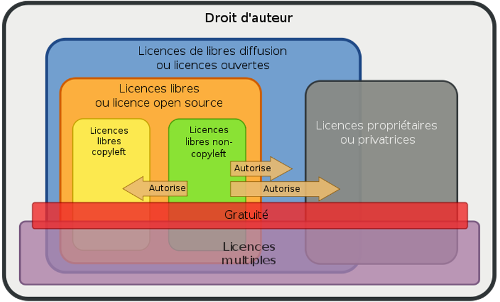
\includegraphics[width=\linewidth]{Figures/wiki-Classification_licences}
                \subcaption{Organisation générale des Licences}
                \label{fig:class_licence_G}
            \end{minipage}
            \hfill
            \begin{minipage}{0.475\linewidth}
                \centering
                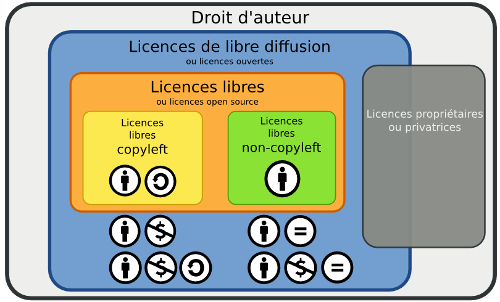
\includegraphics[width=\linewidth]{Figures/wiki-Classification_licences__CC}
                \subcaption{Différents types de licences CC}
                \label{fig:class_licence_CC}
            \end{minipage}
            \hfill
            \newline\strut\newline\centering
            \begin{minipage}{0.95\linewidth}
                \centering
                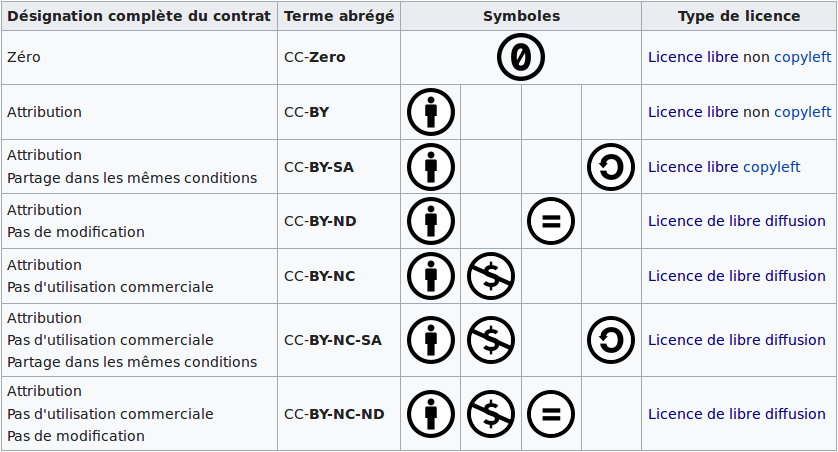
\includegraphics[width=\linewidth]{Figures/wiki-licenceCC}
                \subcaption{Licences CC, leurs codes et leurs symboles}
                \label{fig:tab_licence_CC}
            \end{minipage}
            \caption[Classification des licences]{Schéma de classification des licences (crédit Wikidédia)}\label{fig:class_licence}
        \end{figure}
        \paragraph{La licence \cro{Ouverte}}
            Cette terminologie a été proposée, en 2011, par: la commission sur la mise à disposition ouverte des œuvres de l'esprit par le Conseil supérieur de la propriété littéraire et artistique (CSPLA), du ministère de la Culture français, afin de distinguer ces licences des licences dites \cro{libres}, qui, elles, accordent dans leur définition la plus stricte la totalité des quatre libertés. Cette licence permet de reproduire, rediffuser, adapter et exploiter les données (à condition de mentionner la paternité de l'information). De plus, elle sous-tend la mission \textit{etalab}~\citeURL{etalab} qui, le 18 octobre 2011, publie la Licence Ouverte qui s'appliquera à l'ensemble des réutilisations de données publiques issues des administrations Françaises. Enfin, elle est compatible avec d'autres licences comme l'\textit{Open Government Licence}, son pendant au Royaume-Uni, ou plus généralement avec la licence \sht{CC}\textit{-BY}.
        \paragraph{Licence et type de contenu}
            \strut\addcontentsline{toc}{subparagraph}{Les idées}
                Toutes ces licences ne sont pas applicables à l'ensemble des types de contenus existant. D'une part, il est précisé qu'une idée, un concept, ou un mot ne peut faire l'objet d'une propriété et par extension d'une licence. Cependant, la frontière est parfois floue comme par exemple avec le cas des néologismes. 
            \myPhantom{subparagraph}{Les data}
                Un autre type de contenu faisant office d'exception dans le principe de création d'\gui{œuvres de l’esprit originales} concerne les données ou \textit{data}: sont-elles la propriété de l'individu qui les produit ou de celui qui les recueille. Ce dilemme continue de faire débat et plusieurs éléments d'explication seront fournis dans la suite de ce document~\citeS{sec:data}.
            \myPhantom{subparagraph}{L'audio-visuel}
                Concernant les contenus plus traditionnels: ressources littéraires, documentaires, vidéos, audio, \etc, la majorité des licences sont applicables. 
            \myPhantom{subparagraph}{Le numérique}
                Seuls les logiciels et matériels font l'objet d'un statut un peu particulier du fait qu'ils soient plus apparentés aux inventions (et donc au brevet) qu'aux \gui{œuvres de l’esprit originales}. 
                \begin{table}[!h]
                \begin{minipage}{0.6\linewidth}
                    \centering
                    \small
                    \begin{tabular}{|c|p{1.4cm}|l|}
                        \hline
                        \textbf{Ressource} & \textbf{Logo} & \textbf{Dénomination} \\ \hline\hline
                        Marque (nom et logo) & \vspace{-0.45\baselineskip}
\includegraphics[height=0.8\baselineskip]{Figures/logo-copyright} & Copyright \\ \hline
                        Hardware & \vspace{-0.45\baselineskip}
\includegraphics[height=0.8\baselineskip]{Figures/logo-cc-by-sa} & CC-BY-SA \\ \hline
                        Software &  \vspace{-0.45\baselineskip}
\includegraphics[height=0.8\baselineskip]{Figures/logo-gplv3} & GPLv3\\ \hline
                        Séquences pédagogiques & \vspace{-0.45\baselineskip}
\includegraphics[height=0.8\baselineskip]{Figures/logo-cc-by} & CC-BY  \\ \hline
                    \end{tabular}
                    \caption{Licences Poppy-Project}\label{tab:poppy_licence}
                \end{minipage}
                \begin{minipage}{0.375\linewidth}
                \myDefautStyle
                \myPhantom{subparagraph}{Licence Poppy}
                Pour les besoins du Projet Poppy, 4 types de contenus ont nécessité une mise sous licence: la marque (qui est le nom \textit{Poppy}), les ressources logicielles, matérielles et pédagogiques.
                \end{minipage}
                \end{table}
    \subsection{Les effets collatéraux}\label{sec:com-open}
        \myPhantom{paragraph}{Introduction}
            Le fait d'avoir des contenus, des ressources, et autres plateformes sous des licences ouvertes induit une plus grande accessibilité. Une masse plus importante d'individus passe de simple utilisateur à expert voire même \textit{bidouilleur}\footnote{personne qui répare, créé ou encore trafique un objet, un matériel de manière artisanale, avec des outils qui ne sont pas forcément adaptés} ou développeur. Ainsi, de cette massification, émerge des communautés.
        \subsubsection{Les communautés}
            La communauté open-source est considérée comme une communauté de pratiques, c'est à dire que les personnes qui en font partie sont spécialistes dans un domaine et cherchent dans un but commun à développer, améliorer, maintenir un logiciel, et qui plus est, un logiciel libre. 
            \paragraph{Une plateforme décentralisée et auto-gérée}    
                Les personnes de cette communauté sont amenées à interagir avec d'autres individus, possiblement membres d'autres communautés intéressées par le sujet. Plus la communauté grossit, plus elle devient autonome, et la gestion du projet se retrouve de plus en plus éclatée.
                D’après Ubéda, dans \textit{Logiciels et objets libres - animer une communauté autour d'un projet ouvert}, les communautés sont vitales pour la pérennité des projets de développement logiciel:  
                \citeAtion{ubeda2016logiciels}\par%
                Ils précisent qu’une autre caractéristique essentielle des communautés est de produire des connaissances nouvelles et de stimuler l’innovation, le partage d’informations  et  de  connaissances,  ainsi  que  les  interactions au  sein du groupe permettent de faire émerger des idées, de lancer de nouvelles pratiques, de faire naître des usages en rupture. 
                Plus la communauté s’étend et se diversifie, plus elle devient un gage de qualité et de dynamisme. 
                Les interactions d'une communauté peuvent avoir lieu à la fois sur le web et sur le terrain. 
            \paragraph{Une communauté physique et virtuelle}
                Sur le terrain, les interactions réelles permettent les partages et les échanges tout en faisant connaître le projet pour développer la communauté d'utilisateurs. Dans notre cas, elles permettent aussi d'accompagner les usages~\citeS{sec:reunion} et de les diffuser~\citeS{sec:stand}.
                Sur le web, l’organisation (le rôle de l’équipe principale, les méthodes de prise de décision, de développement et de partage \etc) et les outils d’animations~\citeS{sec:mail} constituent l’architecture de participation de la communauté~\citeB{ubeda2016logiciels}. Il semble donc nécessaire de sélectionner des outils susceptibles de répondre aux besoins et de créer une vitrine numérique (souvent sous forme de site internet) pour que l'utilisateur y accède facilement. 
            \paragraph{Un noyau de contributeurs}
                Il existe différents profils au sein d'une même communauté: certains simples utilisateurs, d'autres diffuseurs, d'autres encore contributeurs parfois occasionnels parfois récurrents, à titre bénévole ou au contraire salarié, tous possèdent un intérêt commun qui se concrétise par la formation de cette communauté, mais chacun possède ses propres besoins et contraintes.
                Lorsque la communauté grandit, le facteur de croissance est souvent spécifique à un profil. Ainsi la population de simples utilisateurs (et leurs demandes) croit plus vite que la population de contributeurs aptes à répondre à leurs demandes. 
        \subsubsection{Réutilisation et dérivations}\label{sec:re-use}
            Le développement de l'Open Source a permis de créer et de diversifier les usages liés à leur contenu. La législation a dû évoluer et différents modèles économico-commerciaux sont venus s'y greffer. 
            Dans le cadre de la réutilisation et de la dérivation nous pouvons distinguer des profils, des objectifs ou des intentions qui sont différentes.
            \paragraph{Par des professionnels ou des amateurs} 
                Plusieurs groupes commerciaux (\ie les \sht{GAFAM}) se partagent le secteur du numérique et jonglent entre les différentes licences pour exploiter au mieux les ressources disponibles. 
                Mais la majorité des réutilisations sont réalisées par des amateurs cherchant à répondre à un besoin très spécifique, qu'il soit professionnel ou personnel. Ces cas de réutilisation/ dérivation sont rarement rediffusés ou même documentés d'où la difficulté de les quantifier précisément.
            \paragraph{Pour un usage personnel ou communautaire}
                L'usage à vocation personnelle est majoritaire chez les utilisateurs, mais le besoin auquel vient répondre cet usage se retrouve probablement chez d'autres utilisateurs. Ce fait est de plus en plus acquis chez les internautes, et il est de plus en plus fréquent de retrouver, sur des forums ou des blogs personnels, des utilisateurs partageant leurs réalisations \gui{pour le plaisir du partage}. Ce comportement est typique de l'émergence d'une culture du partage, favorisé par l'acculturation du grand public au numérique (et des réseaux sociaux).
            \paragraph{Par passion ou par intérêt}
                La création de nouvelles ressources (issues de ressources open source pré-existantes) se développe.
                Mais, de prime abord, une communauté et ses membres partagent, à différents degrés, un intérêt commun: utiliser, maintenir ou développer une même plateforme, par passion ou par intérêt. Dans toute communauté open source nous retrouvons un noyau de passionnés, mais pour la majorité des utilisateurs, ce qui est recherché est avant tout un intérêt pratique d'usage, d'une ou plusieurs fonctionnalités offertes par la plateforme.\par%
                Aujourd'hui, avec l'accroissement des compétences de la population en termes de maîtrise des outils numériques, les consommateurs sont moins naïfs sur les fonctionnalités réelles des différentes plateformes.
                Ainsi, de nombreux utilisateurs de produits commerciaux se sont orientés vers des solutions Open Source. Par exemple, de plus en plus d'enseignants privilégient l'installation et l'usage de la suite logiciels Libre Office au détriment de Microsoft Office.\par%
                En réponse à cela, certains industriels du numérique ont adapté leur stratégie et plusieurs fusions-acquisitions récentes dans le secteur font craindre sur le devenir des communautés open source. Par exemple, l'acquisition de GitHub par Microsoft pour 7,5 milliards de dollars, l’acquisition de Mulesoft par SalesForce pour 6,5 milliards de dollars et le rachat de Red Hat par IBM pour 34 milliards de dollars qui figurent parmi les plus importantes acquisitions de l'histoire du secteur informatique.
                Ainsi, les fournisseurs de logiciels open source sont incités à protéger leur code contre les sociétés qui poursuivent uniquement un objectif marketing monétisant ce qui devrait être librement disponible.
                Par exemple, Amazon a tiré profit du logiciel de Redis Labs sans contrepartie pour la communauté open source. En réaction, Redis Labs a créé une nouvelle licence logicielle imposant des restrictions claires sur ce qu’il est possible de faire avec son logiciel, et ce qui ne l’est pas.
                Mais, de fait, cela limite la possibilité pour les entreprises d’enrichir, de contrôler et de contribuer aux projets, créant ainsi un cercle vicieux à l'encontre de la philosophie Open source mais qui semble nécessaire à sa survie. 
                Avec de tels changements de posture dans ce secteur, l'open source peut-il vraiment rester \gui{open}? La naissance d'associations comme la Continuous Delivery Foundation montre une volonté de maintenir cette façon de travailler, d’œuvrer et de collaborer pour le bien commun. Pourtant, la question se pose: dans la mesure où les entreprises imposent des restrictions sur leurs logiciels pour protéger leurs communautés, l’open source est-il encore vraiment \gui{open}? Faut-il même laisser ces entreprises imposer des restrictions? Qui a l’autorité de prendre une telle décision?
\section{La robotique éducative}
    \myPhantom{paragraph}{Introduction}
        Il existe plusieurs exemples dans la littérature sur la possibilité d'utiliser un robot comme outil pédagogique~\citeB{benitti2012exploring, baron1994informatique}. De nombreux robots sont développés et des études ont été réalisées pour tester l'amélioration de la transmission de connaissances dans ce cadre.
        La robotique pédagogique est une robotique bien particulière. Elle a des caractéristiques qui la distingue des autres types de robotique. Mais dans un premier temps, qu'est ce qu'un robot?
        \myPhantom{subparagraph}{Origine du robot}
            Le terme robot est issu des langues slaves et formé à partir du radical rabot, rabota (en russe) qui signifie travail, corvée que l'on retrouve dans le mot Rab, esclave en russe. Il fut initialement utilisé par l’écrivain tchécoslovaque Karel Čapek dans sa pièce de théâtre R.U.R. (Rossum's Universal Robots) en 1920. Mais de tous temps, l’homme a cherché à se faire remplacer pour des tâches spécifiques pouvant être dangereuses, rébarbatives, longues ou répétitives. Ainsi, il faut remonter jusqu’à la préhistoire pour trouver les premiers automatismes avec les premiers pièges. Ainsi, un collet à déclencheur est un bon exemple de mécanisme doté d’un détecteur et d’un actionneur.
            Les ancêtres des robots sont les automates. Les plus anciennes sources de réalisations concrètes semblent réalisées par l'inventeur arabe Al-Jazari au \siecle{12}. Un automate très évolué fut présenté par Jacques de Vaucanson en 1738: il représentait un homme jouant d’un instrument de musique à vent. Jacques de Vaucanson créa également un automate représentant un canard mangeant et refoulant sa nourriture après ingestion de cette dernière.
            Mais qu'appelle-t-on robot aujourd'hui?
        \myPhantom{subparagraph}{Définition d'un robot}    
           \citeAtion{robot-Oxford}
            Une machine capable d’effectuer automatiquement une série complexe d’actions, en particulier quand elle peut être programmée par un ordinateur, semble être une définition plutôt succincte, mais elle reflète l'absence de consensus actuel sur la définition de robot: certaines trop laxistes permettent d'inclure tout mécanisme (\eg un collet) ou, au contraire, d'autres trop restrictives excluant des artefacts pourtant communément admis comme étant des robots. L'\sbg{ife} proposait en 2017 cette définition:
           \citeAtion{robot-ife}
            Bien que plus précis, notamment en intégrant 4 des 5 composants essentiels à la constitution d'un robot: énergie, capteur, actionneur, micro-contrôleur et structure~\citeS{sec:5compo} et en mentionnant les aspects de programmation; elle néglige les questions d'adaptation à l'environnement et les boucles de retro-action faisant émerger le comportement robotique.\par% 
        \myPhantom{subparagraph}{Définition d'un comportement robotique}
            Le comportement d'un robot ne se réduit pas au programme contenu en lui, mais se déduit par l'observation du code plongé dans un environnement physique. Pour s'exécuter, ce programme aura besoin d'un corps (d'un robot) pour incarner ce programme: un même programme ne produira pas le même comportement sur deux robots structurellement différents. Ainsi, le comportement d'un robot est déterminé par son programme, sa structure physique et l'environnement dans lequel il évolue. Plus, l'un ou l'autre, de ces déterminants est complexe moins le comportement correspondra à la somme de ceux-ci. On parle alors de comportement émergeant.\par%
        La robotique pédagogique a pour vocation de faire naître un intérêt pour ces notions et de les transmettre chez un public très large.
        Elle a donc pour cible une catégorie de la population qui n'est pas professionnelle du domaine. Cela peut être des adultes mais aussi en grande partie des enfants (dans le cadre scolaire ou non).
        À l'instar des mathématiques enseignés dans les cycles inférieurs sans volonté absolue de créer des mathématiciens, la robotique pédagogique se place comme un enseignement général permettant d'offrir une culture commune, des bases de communication et de réflexion autour de la notion de robot et d'algorithme.
        Cela engendre des besoins qui lui sont propres. Pour répondre à ces besoins, différents types de robots éducatifs existent et se complètent.
    \subsection{Les origines}
        \paragraph{Logo}
            Sur le plan informatique, Logo est un langage de programmation orientée objet réflexif~\citeB{harel1990software}. Principalement connu pour sa tortue graphique, il était également en mesure de manipuler des listes, des fichiers et des entrées/sorties, certaines fonctionnalités étant plus avancées que sur d'autres langages de la même époque, comme Basic ou Pascal\footnote{deux langages de programmation à visée éducative}.
            Mais le terme Logo renvoie également à la mise en pratique par Seymour Papert d'un mode d’apprentissage inspiré des travaux de Jean Piaget sur le développement cognitif de l’enfant~\citeB{ackermann2001piaget}. Papert propose de créer de nouveaux supports qui pourront être manipulés par les enfants, des matériaux qui soient propres à favoriser l’acquisition de notions comme les mathématiques, la physique, \etc, grâce à la démocratisation de l’informatique et de la robotique. Il redéfinit le concept d'erreur en éducation~\citeS{sec:erreur}, en la qualifiant comme un défaut partiel et momentané dans un programme \gui{un simple bug informatique} à identifier et, le cas échéant, à corriger. Il développe l'idée du micromonde d'apprentissage nommé \cro{mathématie} et énonce 3 principes fondamentaux à l'apprentissage naturel:
            \begin{itemize}\myItemStyle
                \item le principe de continuité, continuité avec les connaissances déjà bien assimilées par les enfants, ce qui permet un ancrage cognitif et un possible rapport affectif
                \item le principe de puissance ajoutée, qui permet à l’enfant, grâce à ses nouvelles connaissances, de développer de nouveaux projets chargés de significations personnelles 
                \item le principe de résonance culturelle, par laquelle les mathématiques apprises par les enfants trouvent un sens dans un contexte social car, pour pouvoir en avoir un à leurs yeux, il faut qu’elles en aient également aux yeux des adultes.
            \end{itemize}{}\par%
            Papert a été un précurseur tant en informatique qu'en pédagogie, il est aujourd'hui encore régulièrement cité pour ses travaux sur Logo qui, malgré l'évolution dans le domaine, reste d'actualité.
            \begin{figure}[!h]
                \centering
                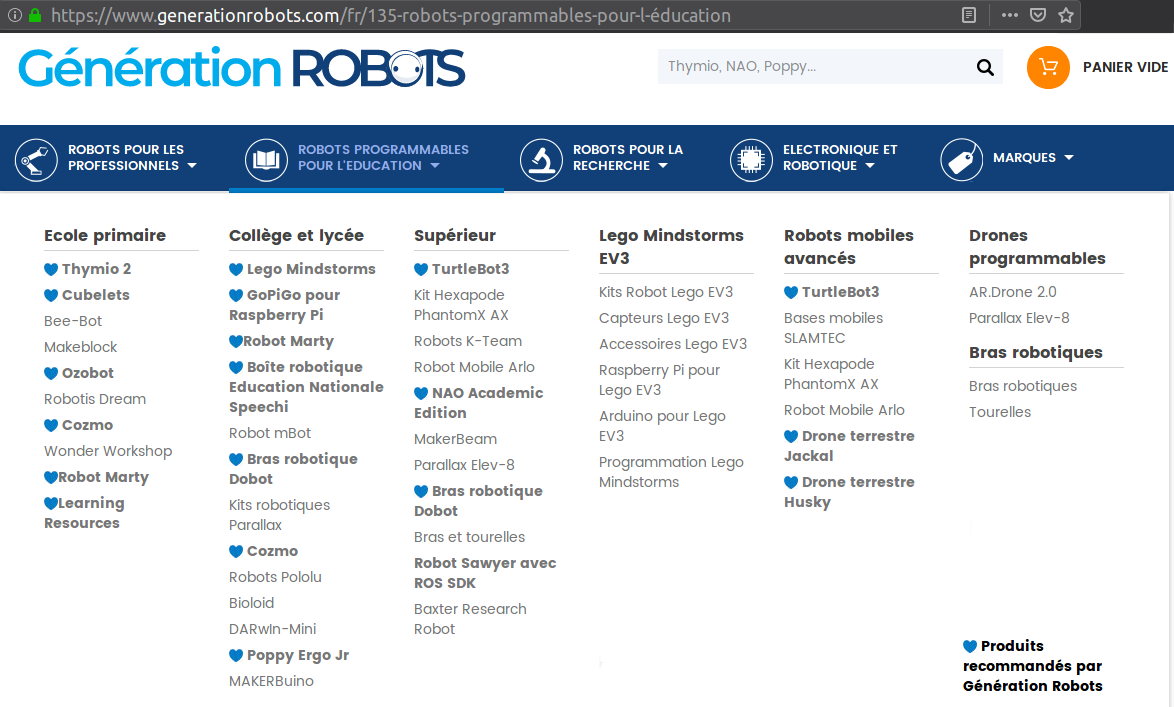
\includegraphics[width=0.9\linewidth]{Figures/bot-GR}
                \caption{Catalogue en ligne Génération Robot}\label{fig:list_bot}
            \end{figure}
        \paragraph{Aujourd'hui}
            Robotique éducative et robotique pédagogique sont à distinguer~\citeURL{ife_robotique_2017}, la première regroupe l'ensemble des utilisations des robots dans le milieu de l'éducation. Tandis que la seconde ne concerne que l'utilisation des robots à des fins d'enseignement (de la programmation, de l'algorithmique et autres connaissances se rapprochant de l'informatique). Mais toutes deux sont utilisées dans l'enseignement, de la maternelle à l'enseignement supérieur. Chaque robot possède ses caractéristiques qui lui permettront de s'insérer dans l'une ou l'autre de ces catégories.
	        %Son utilité est démontrée en 2007 dans le cadre d'une classe d'école élémentaire américaine~\citeB{barker2007robotics}
    \subsection{Caractéristiques générales}
        \myPhantom{paragraph}{Introduction}
            Le mode de déplacement du robot, le code qui en découle, ou la façon d'appréhender ses mouvements seront directement dépendants de sa forme qui lui est propre. Cependant, il existe plusieurs grands types de locomotions, plus ou moins complexes qui seront sélectionnés en fonction du but que l'on se fixe (\eg être capable d'avancer sur un terrain accidenté). Les mouvements du robot peuvent être plus ou moins perfectionnés et le choix du type de locomotion du robot influence ses autres possibilités de déplacement.
        \subsubsection{La mobilité}
            \begin{figure}[!h]
                    \centering
                    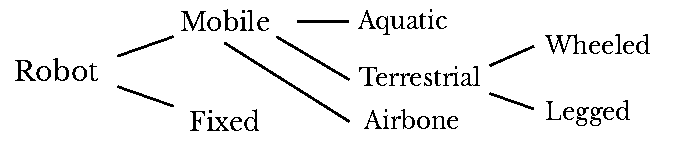
\includegraphics[width=0.8\linewidth]{Figures/Mondada-classification.pdf}
                    \caption{Classification type de locomotion robotique, Ben-Ari~\citeB{ben2018elements}}
                    \label{fig:Classification}
            \end{figure}\par%
            \myPhantom{paragraph}{Introduction}
                Il existe plusieurs moyens de locomotions utilisés en robotique. Un moyen communément utilisé, simple et intuitif, est le déplacement sur roues. Cependant, ce moyen peut devenir un peu limitant dans certaines situations notamment en terme de franchissement. Un autre moyen courant est l'utilisation de pattes. Néanmoins, il existe d'autres types de déplacements comme, par exemple, les roues pattes (une combinaison entre les pattes et les roues), ou encore les chenilles.
                La catégorie cinématique qui en découlera contraint les caractéristiques du robot en terme de manœuvrabilité et de stabilité. Ainsi, chaque catégorie possédant ses avantages et inconvénients, le choix de la configuration du robot doit être réalisé en fonction de l'usage attendu.
            \paragraph{Les robots à base fixe}
                Les robots fixes sont principalement des bras robotiques manipulateurs utilisés dans l'industrie dans des environnements bien définis et des tâches répétitives spécifiques, telles que la peinture de pièces dans des usines de fabrication automobile, la fixation de boulons, \etc. Les bras robotiques peuvent être utilisés à des fins de robotique collaborative: le bras assiste directement le geste de l'opérateur en multipliant ses capacités en termes d'efforts pour manipuler en toute sécurité des objets chauds, lourds ou volumineux, ou au contraire trop petit pour être saisis naturellement avec la précision nécessaire, tout en s'adaptant aux caractéristiques de l'utilisateur et à ses mouvements. Grâce à l'amélioration des capteurs et des dispositifs d'interaction homme-robot, les manipulateurs robotiques sont de plus en plus utilisés dans des environnements moins contrôlés, tels que les chirurgies de haute précision.
                En terme de programmation et dans le but de faire se déplacer ce bras, il faut avant tout être capable d'estimer les angles des articulations nécessaires pour imposer une certaine position de l'extrémité du bras, et inversement, estimer la position de l'extrémité du bras en fonction de l'état des articulations.
                \begin{figure}[!h]
                \begin{minipage}{0.55\linewidth}
                    \centering                    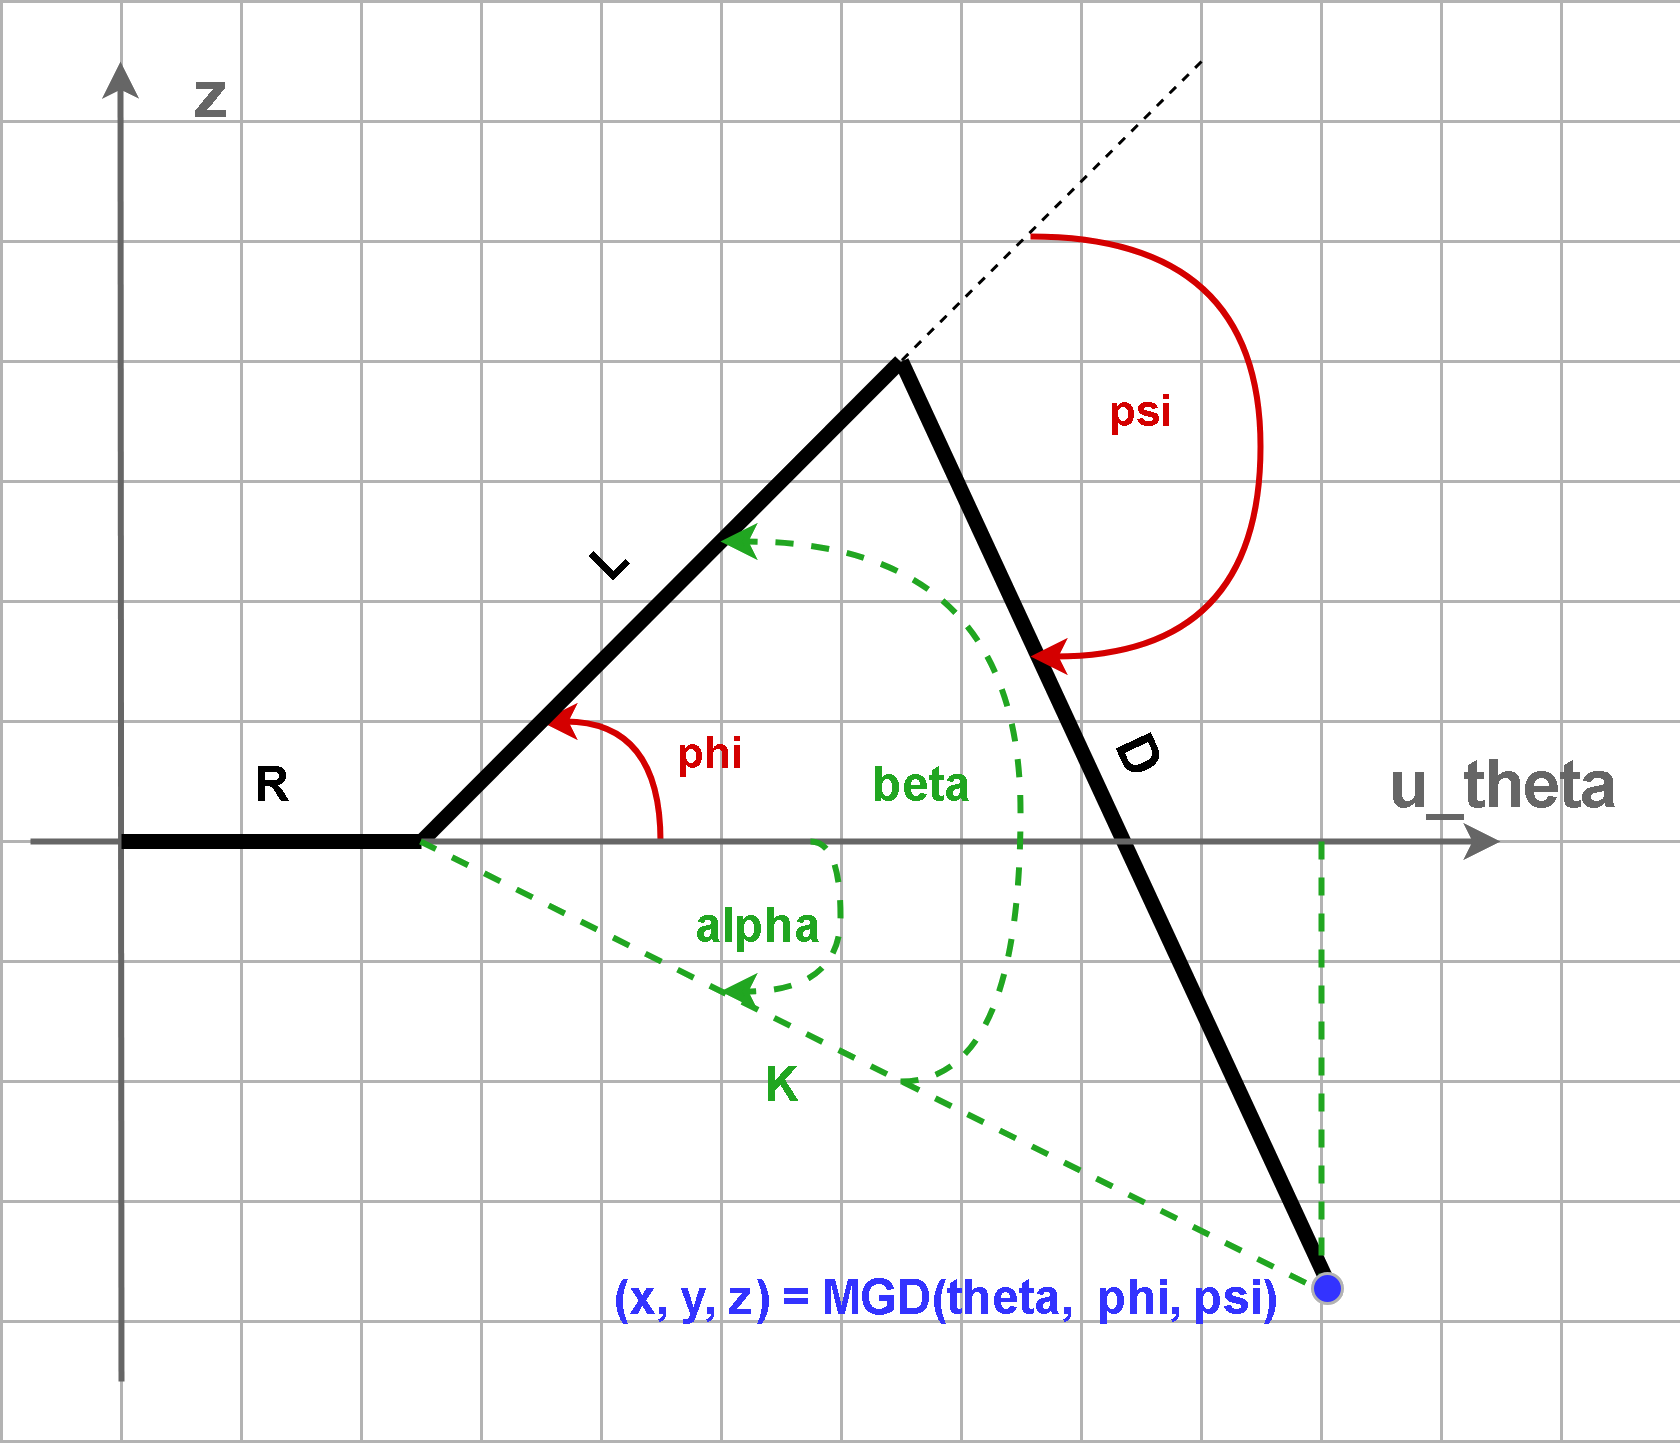
\includegraphics[width=0.9\linewidth]{Figures/geo_leg}
                    \caption{Modèle géométrique d'une patte}\label{fig:geo_leg}
                \end{minipage}
                \hfill
                \begin{minipage}{0.425\linewidth}
                \myDefautStyle
                De manière théorique, nous pouvons aborder le raisonnement de manière similaire aux calculs appliqués pour une patte articulée.
                \subparagraph{Modèle géométrique direct}
                    Le modèle géométrique direct consiste à calculer les coordonnées $(x, y, z)$ de l'extrémité d'une patte, connaissant chacun de ses angles $(theta, phi, psi)$.
                \end{minipage}
                \end{figure}
                \subparagraph{Modèle géométrique inverse}
                    Le modèle géométrique inverse, consiste à trouver des angles $(theta, phi, psi)$ permettant de placer l'extrémité de la patte aux coordonnées $(x, y, z)$ voulues. Il n'existe pas forcément de solutions, ni de solution unique.
                    %La méthode \texttt{MGI} de la classe \texttt{DiploLeg} calcule une solution, et renvoie un résultat s'approchant le plus possible de la commande désirée, lorsque celle-ci est géométriquement impossible à atteindre. L'angle $theta$ est triviallement calculé à partir de $x$ et $y$. Pour obtenir les angles $phi$ et $psi$, des calculs intermédiaires sont nécessaires. La figure \ref{fig:leg_de_cote} montre en vert les variables intermédiaires utilisées. On utilise le théorème d'Al-Kashi, permettant de calculer les angles d'un triangle dont on connaît les longueurs des côtés. Ainsi, on obtient $psi$ à partir du triangle de longueurs $(L, D, K)$. Du fait de la non unicité des solutions, on impose $psi < 0$ afin d'obtenir une disposition de patte adaptée à la marche. De la même manière, $phi$ est obtenu à partir de deux angles intermédiaires, $alpha$ et $beta$, calculés respectivement grâce à $(z, K)$ et le triangle de longueurs $(L, D, K)$.\\
                    Ainsi, il est possible grâce à cette méthode de traduire une commande sur les coordonnées cartésiennes de l'extrémité de la patte (dans un repère lié au robot)  en commande sur chaque angle des moteurs.
            \paragraph{Les robots à roues}
                Les robots à roues sont les plus répandus de nos jours. Ce moyen de locomotion, certainement l'un des plus répandu de nos jours, est optimal dans les environnements créés par l'homme, mais plutôt mal adapté aux milieux présentant des irrégularités ou obstacles à franchir.
                Mais, en comparaison à d'autres modalités de déplacement, les robots à roues possèdent l'avantage d'avoir un modèle cinématique simple. La configuration des roues reste néanmoins importante pour la manœuvrabilité et la stabilité du robot, comme le montre Bayle~\citeB{bayle2008robotique}.
                \begin{figure}[!h]
                    \centering
                    \begin{subfigure}{0.225\linewidth}
                    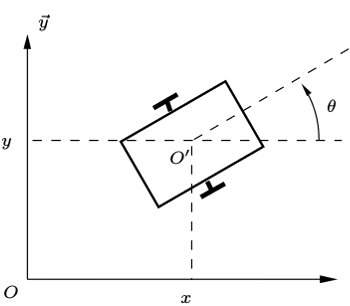
\includegraphics[width=\linewidth]{Figures/Bayle-type_de_roue-a}
                    \subcaption{Unicycle}\label{fig:bot_roue-a}
                    \end{subfigure}
                    \begin{subfigure}{0.225\linewidth}
                    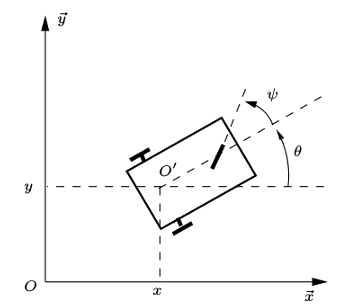
\includegraphics[width=\linewidth]{Figures/Bayle-type_de_roue-b}
                    \subcaption{Tricycle}\label{fig:bot_roue-b}
                    \end{subfigure}
                    \begin{subfigure}{0.225\linewidth}
                    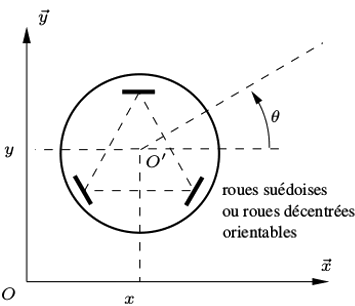
\includegraphics[width=\linewidth]{Figures/Bayle-type_de_roue-c}
                    \subcaption{Omnidirectionnelle}\label{fig:bot_roue-c}
                    \end{subfigure}
                    \begin{subfigure}{0.235\linewidth}\raggedright
                    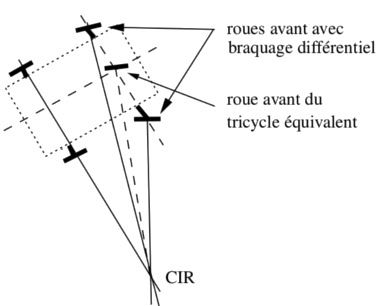
\includegraphics[width=\linewidth]{Figures/Bayle-type_de_roue-d}
                    \subcaption{Équivalence}\label{fig:bot_roue-d}
                    \end{subfigure}
                    \caption[Robot à roues, Bayle~\citeB{bayle2008robotique}]{Grandes catégories de disposition de roues, Bayle~\citeB{bayle2008robotique}}\label{fig:bot_roue}
                \end{figure}\par%
                Pour calculer et estimer les déplacements du robot il faut que la géométrie de celui-di impose à tout instant un unique point fixe autour duquel tourne le robot, nommé Centre Instantané de Rotation (CIR). Cette dernière contrainte limite le nombre de configurations possibles à trois catégories principales, schématisées par la figure~\ref{fig:bot_roue}: les robots de type unicycle, tricycle, et omnidirectionnel.
                Chacune de ces catégories englobe un ensemble de robots pouvant posséder un nombre de roues différent, mais dont la géométrie est équivalente d'un point de vue cinématique. Par exemple, le 4\ieme élément de la figure~\ref{fig:bot_roue-d} montre l'appartenance des robots de type voiture (à géométrie d'Ackermann) à la catégorie des tricycles. Un point crucial pour l'odométrie est l'adhérence des roues au sol car les pertes d'adhérence sont trop aléatoires pour être prises en considération durant le calcul.
                \subparagraph{Robots unicycles}
                    Ce type de locomotion~\citeF{fig:bot_roue-a}, très répandu du fait de sa simplicité cinématique, permet d'imposer facilement au robot une vitesse longitudinale et angulaire à partir des moyennes et différences de vitesse de rotation de ses deux roues motrices. Mais, ces robots peuvent poser des problèmes de stabilité et il est commun d'y ajouter une troisième roue folle en dehors de l'axe des roues motrices.
                \subparagraph{Robots tricycles}
                    Les robots de la catégorie tricycles~\citeF{fig:bot_roue-b} sont très peu stables. En pratique, on utilise des robots à quatre roues de la même classe cinématique: les robots à géométrie de type Ackermann. Comme montré en figure~\ref{fig:bot_roue-d}, la géométrie Ackermann, celle des voitures, consiste à utiliser deux roues avant pivotantes, mais dotées d'un braquage différentiel, afin que leurs axes de rotation se croisent avec celui des roues arrières en un seul point. On obtient ainsi un robot à grande stabilité mais d'une faible manœuvrabilité.
                \subparagraph{Robots omnidirectionnels}
                    Cette catégorie offre la plus grande manœuvrabilité pour le robot car il est possible d'agir indépendemment sur les deux vitesses de translation et sur la vitesse de rotation. Cependant, elle engendre une plus grande complexité mécanique, ainsi qu'une odométrie moins fiable.
            \paragraph{Les robots à chenilles et rampants}
                Dans un contexte de mobilité, nous sommes rapidement confrontés au problème du déplacement sur des surfaces inégales et au franchissement d’obstacles. Les robots à chenilles ont l’avantage de proposer des solutions plus faciles à mettre en place que des robots à pattes pour résoudre ce genre de problème, même si plus limités dans leurs usages.
	            Ces robots peuvent prendre différentes formes et avoir différents types de chenilles, Mr Jean-Luc Paillat en a proposé une classification~\citeB{paillat2010conception}. Ainsi il y a des robots à géométries fixes et des robots à géométries variables qui peuvent être soit à chenilles non-déformables, soit à chenilles déformables.
	            D’autres méthodes de la locomotion existent mais sont moins répandues, par exemple, les robots inspirés par les serpents. Ces derniers sont basés sur une structure hyper-redondante qui leur permet différents modes de déplacements, on retrouve en particulier dans la nature l'ondulation latérale, le mouvement en accordéon et le déroulement latéral.
                Concrètement, nous retrouvons des exemples comme les robots \cro{modsnake} développés par des équipes de la Carnegie Mellon University, capables de monter sur une jambe ainsi que réaliser du déplacement latéral et ondulatoire.
                Ou plus basiquement, les robots de Gavin miller dont la deuxième version se déplace par ondulation.
                Ces robots nécessitent des formes et textures particulières si l’on souhaite les voir passer des obstacles. De plus, ils sont beaucoup moins évidents à comprendre en terme de mouvement et de programmation que les robots à roues, chenilles ou pattes.
            \paragraph{Les robots à pattes}\label{sec:mob_patte}
                Un premier point concerne le nombre de pattes à utiliser, puis comment utiliser chaque patte et comment doivent-elles être conçues structurellement afin de pouvoir effectuer des déplacements les plus efficaces tout en restant à un niveau simple d'implémentation. 
                Dans la nature, le nombre de pattes sur lesquelles les animaux se déplacent peut varier de 1 à un millier. Pourtant, malgré cette forte variabilité, des allures similaires sont observées. Cela peut laisser à penser qu'il existe certaines façons de se déplacer avec des pattes qui sont plus efficaces que d'autres.
                \begin{figure}[!h]
                    \centering
                    \begin{subfigure}{0.495\linewidth}
                    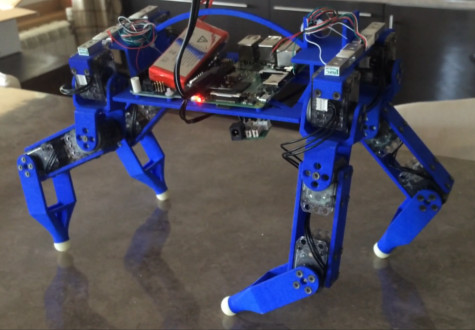
\includegraphics[width=\linewidth]{Figures/bot-quattro.jpg}
                    \subcaption{Quattro, Robotitia~\citeURL{roboticia}}\label{fig:quattro}
                    \end{subfigure}
                    \begin{subfigure}{0.495\linewidth}
                    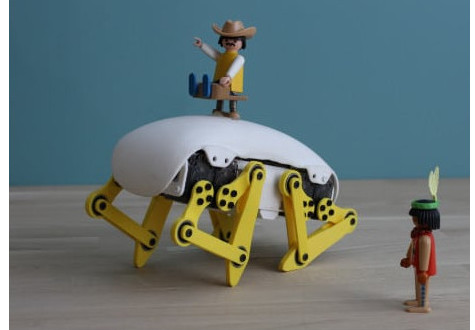
\includegraphics[width=\linewidth]{Figures/bot-doggy.jpg}
                    \subcaption{Doggy, Pollens Robotics~\citeURL{pollens}}\label{fig:doggy}
                    \end{subfigure}
                    \caption[Robot à pattes, Quattro et Doggy]{Deux dérivations de ErgoJr}\label{fig:bot_patte}
                \end{figure}\par%
                Dans la représentation usuelle, une patte se constitue de 3 degrés de liberté. Or, il est tout à fait possible de concevoir une patte avec plus de 3 degrés de liberté~\citeF{fig:geo_leg} ou avec moins comme, par exemple, le mécanisme de Jansen~\citeF{fig:bot_patte}.
                De nombreux robots à pattes existent actuellement. Une catégorie notoire est la catégorie des robots bipèdes comme ASIMO de Honda ou Nao d'Aldebaran. Mais, la marche bipède reste un challenge, entre autres, car le nombre limité de pattes engendre des difficultés au niveau de la stabilité~\citeS{sec:poppy_science}. En terrain accidenté, ces difficultés sont largement augmentées. Certains robots sont construits spécialement afin de pouvoir évoluer sur des terrains extrêmement accidentés comme Big dog et Little dog de Boston Dynamics à 4 pattes.
                Enfin, notons qu'il existe un robot un peu particulier, le Strandbeest de Theo Jansen, un artiste~\citeF{fig:strandbeest}. Ce robot à pattes est fabriqué uniquement avec des tubes en plastique jaune et se déplace grâce à l'énergie du vent sur les plages, sa structure lui permet de détecter l'eau et de l'éviter.
                \begin{figure}[!h]
                    \centering
                    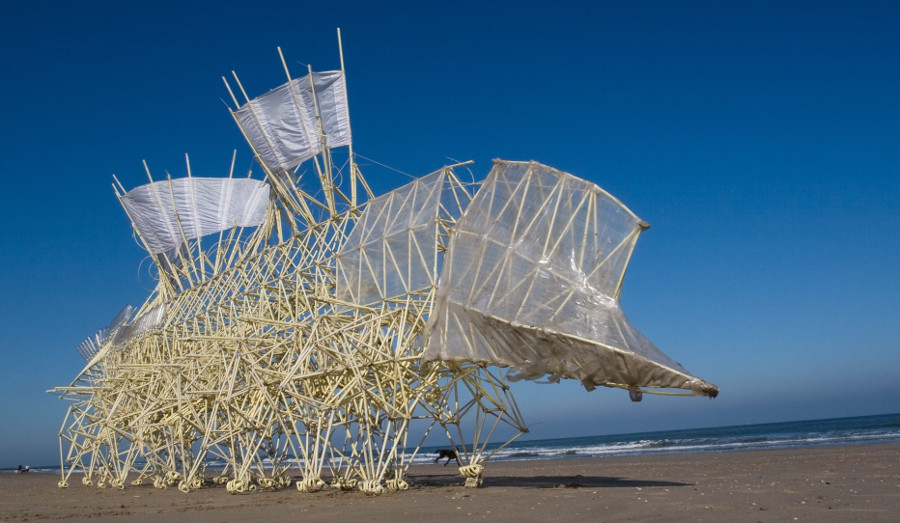
\includegraphics[width=\linewidth]{Figures/bot-standbeest}
                    \caption{Un Strandbeest de Theo Jansen.}\label{fig:strandbeest}
                \end{figure}\par%
                Pour stabiliser ces créatures, il existe des critères génériques (à adapter aux structures spécifiques du robot). Un premier critère est la stabilité statique qui suppose que les mouvements sont suffisamment lents pour négliger les aspects dynamiques. Un autre est le ZMP (Zero Moment Point), qui est un point associable à chaque configuration du robot et qui doit se trouver dans son polygone de sustentation pour assurer sa stabilité.
                Afin de diriger un robot à pattes, chaque robot possède son propre contrôleur qui permet de faire bouger les pattes d'une certaine manière. Dans sa thèse, Grégoire Passault~\citeB{passault:tel-01441799} décrit son contrôleur permettant de diriger les pattes d'un robot à pattes, il teste le contrôleur pour toute une gamme de robots à pattes, en faisant varier le nombre de pattes, l'agencement des degrés de liberté et leur forme.
            \paragraph{Les robots hybrides roues-pattes}
                Il est également possible de combiner pattes et roues, et ainsi pouvoir obtenir des déplacements à grande mobilité, sur des terrains accidentés semés d'obstacles~\citeB{pierre2013optimisation}. En effet, en fonction des propriétés du terrain à parcourir, les robots hybrides peuvent utiliser soit la marche, soit le roulement, mais aussi des modes de locomotion plus complexes, tel que le péristaltisme, consistant en un déplacement de chaque patte, mais sans perte de contact avec le sol. 
                Le franchissement de grands obstacles est aussi possible avec beaucoup plus de facilité que pour des robots à roues, les pattes pouvant franchir une à une l'obstacle tout en maintenant le robot dans une configuration géométrique stable. 
                Mais leur mise en place est complexe et onéreuse.
            \paragraph{Les robots non-terrestres}
                Ce type de robot est relativement peu répandu, notamment dans le domaine éducatif car il nécessite des contraintes environnementales fortes:
                \myPhantom{subparagraph}{Les robots volants} 
                    Les robots volants comme les drônes ont besoin d'un espace suffisamment grand et de conditions climatiques favorables ( \eg peu de vent) même s'il est vrai que la plupart des établissements scolaires disposent d'un gymnase (ou les conditions de vol seraient idéales pour ce type d'engin) les interrogations sur la législation en vigueur dissuadent son utilisation en public ou dans le cadre professionnel. En effet, suite au développement de l'offre grand public, notamment durant la période de Noël, et des usages non prescrits qui en découlent, la question de la responsabilité en cas de dégâts ou simplement en terme d'occupation de l'espace aérien (qui est réglementé) se pose. La loi évolue pour rendre compte de ces nouveaux usages, et rend le processus de développement plus long.
                \myPhantom{subparagraph}{Les robots marins et sous-marins}
                    Un autre exemple d'engins non-terrestres sont les robots marins et sous-marins. Certainement les moins répandus de nos jours, simplement par manque de lieux adaptés à leur utilisation. De plus, du fait de leur éloignement physique durant l'utilisation, ce type de robot se prive d'éléments favorisants les apprentissages tels que l'interaction directe et le rapport à l'erreur~\citeS{sec:tangible}. 
                \myPhantom{subparagraph}{Les robots fusées}
                    Il en est de même pour les robots de type fusée que l'on rencontre dans certains concours locaux.
            \paragraph{Soft Robotique}
                Ou robotique douce en français, est un domaine de la robotique qui traite de robots construits à partir de matériaux souples et déformables capables d’interagir en toute sécurité avec les humains et l’environnement. La compliance et la douceur s'inspirent des organismes vivants. L'utilisation de champs électriques, de polymères thermiques ou de pneumatiques gonflables, permet de mettre en œuvre les principes de l'intelligence incarnée, ou calcul morphologique. Mais, ce domaine reste actuellement une niche principalement exploitée dans le monde de la recherche scientifique et qui connaît encore peu d'applications industrielles ou grand public.
            \paragraph{Swarm robotics}
                Ou robotique en essaim, est une approche de la robotique collective qui s’inspire des comportements auto-organisés d’animaux sociaux. À travers des règles simples et des interactions locales, la robotique Swarm vise à concevoir des comportements collectifs robustes, évolutifs et flexibles pour la coordination d'un grand nombre de robots~\citeB{brambilla2013swarm}.
            \paragraph{Synthèse}
                L'ensemble de ces moyens de locomotion sont aujourd'hui exploités par les robots et ceci peu importe le domaine d'application: industrielle, scientifique, grand public ou éducatif, tous, manipulent, suivant les besoins et dans des proportions variables, tel ou tel type de déplacement.
        \subsubsection{Leurs Formes}\label{sec:forme}
            Concernant les caractéristiques morphologiques du robot, l’article de Chang \& al~\citeB{chang2010exploring} précise que la forme du robot, son apparence et ses agissements peuvent influencer la motivation et l’engagement des élèves. En effet, la flexibilité du robot et son caractère modifiable, peuvent permettre à l’enseignant d’ajuster et de designer un robot approprié aux activités, afin d’avoir un meilleur matériel instructionnel. Les apprenants sont également moins limités. Concernant l’apparence, les auteurs considèrent les robots comme supports pour éveiller la curiosité et l'imagination. L’aspect physique du robot est donc à soigner puisque la motivation joue un rôle important dans les performances d'apprentissage. Enfin, l‘une des fonctions fondamentales des robots est leur capacité à interagir avec des personnes, cet élément est donc essentiel à mettre en avant.
            \paragraph{Animaloïde, ou non}
                L'engagement des élèves est crucial pour l'adoption du robot comme un outil pédagogique efficace. Pour cela, la forme et l'esthétique du robot ont une influence assez importante sur la première impression ainsi que dans la motivation à son utilisation.
                % Certaines formes avec des lignes brutes, carrées vont par exemple favoriser un public masculin, renvoyant à l'image de robot
                Une forme anthropomorphique ou zoomorphique va susciter au premier regard une intention, et va faire référence à un imaginaire déjà  nourrit par la science fiction et les a-priori. Cet imaginaire peut être positif (\eg Astro Boy) ou négatif (\eg mythe du robot tueur ou de skynet), ce qui va dans le premier cas poser des attentes très élevées difficilement réalisables et ainsi amenant facilement à une déception et dans le second cas un rejet au premier abord. Tenter de s'absoudre de ces conceptions initiales en privilégiant une forme neutre semble une option plus adéquate dans un but de diffusion générique. Ou, au contraire, forcer certains traits tout en s'assurant que les attentes ainsi générées par ceux-ci seront satisfaites.
            \paragraph{Les robots bio-inspirés}
                C'est l'objectif de ce type de robot fabriqués en se basant sur le modèle d'un animal vivant. Le but alors n'est pas forcément qu'il soit capable de reproduire l'ensemble des compétences de l'animal qu'il mime, mais de satisfaire les attentes qu'il génère:. c'est le cas de robots pédagogiques tels que Metabot capable de tout franchir tel une araignée; le robot bionicAnts reproduit le caractère collaboratif entre fourmis; AIBO, le chien, est quant à lui un robot de compagnie.
            \paragraph{Modifiable, ou non}
                Avec l'accessibilité croissante des outils de conception et de production~\citeS{sec:3D_print}, créer sa propre créature ou objet robotique devient une possibilité pour un grand nombre d'individus. De plus, des robots comme les Mindstorms, Kibo ou les robots Poppy~\citeS{sec:bot} propose d'emblée de pouvoir adapter ou modifier le kit d'origine ou même d'en créer un nouveau. Dès lors, l'utilisateur passe de simple usager à concepteur, changeant son rapport à la discipline robotique, largement pluri-disciplinaire~\citeS{sec:pluri_bot}, et au robot en lui-même notamment en terme d'interaction. 
        \subsubsection{Interaction}
            \paragraph{Support physique}
                Par exemple~\citeS{sec:bot}, le robot Thymio propose au démarrage un set de 6 comportements pré-programmés représentés par des couleurs, celles-ci permettent une première approche du robot. À l'instar de Bee-bot, Il est possible (dans sa couleur violette) d'orienter les déplacements de Thymio grâce aux flèches directionnelles sur sa face supérieure. Blue-bot offre, lui, plus de possibilités grâce à un clavier de commandes permettant de programmer le robot à l’aide de cartes représentant une action à effectuer. Les enfants insèrent les cartes dans un certain ordre dans un clavier de commandes, et observent ensuite le robot réaliser chaque instruction dans l’ordre. 
                Ces 3 robots utilisent donc ici un support physique. L’utilisation d’un tel support pour la programmation du robot est indispensable pour les plus jeunes, pour qui l'utilisation d'une interface numérique reste une barrière car relevant d'un niveau d'abstraction supplémentaire qui requière un apprentissage à part entière.
                Cependant, pour offrir des possibilités de programmation large et flexible, l'intermédiaire d'un langage spécifique de plus ou moins haut niveau sera indispensable.
            \paragraph{Support numérique}
                Sur la forme, il nécessite une interface numérique (\eg un ordinateur, une tablette, \etc).
                Sur le fond, il peut s'agir d'une simple interface de contrôle jouant des programmes pré-enregistrés~\citeS{sec:monitor}, ou d'applications plus complexes permettant d'illustrer certains rudiments de programmation~\citeS{sec:VPL}, ou, au contraire, de langage à proprement parlé, permettant d'exploiter le maximum des capacités du robot.
    \subsection{Les Langages}
        De nombreux langages de programmation existent, Wikidédia les recense et en comptabilise plusieurs centaines~\citeURL{list_lang}. Tous ont des propriétés propres et sont utilisés dans des domaines spécifiques pour lesquels ils ont été développés.
        \myPhantom{paragraph}{Langue bas niveau}
            Il existe des langages dits de bas niveau qui requièrent une connaissance précise du fonctionnement de la machine et qui permettent de manipuler explicitement les éléments physiques, la mémoire par exemple. Un exemple de ce type de langage est le langage assembleur.
        \myPhantom{paragraph}{Langue haut niveau}
            Il existe des langages qui ne nécessitent pas une connaissance poussée du fonctionnement de la machine et qui sont plus proches du langage naturel, on parle de langages de haut niveau. Ces langages, comme Python, permettent d'écrire des programmes plus facilement, mais ils requièrent des connaissances particulières sur le langage en lui-même, telles que les règles de syntaxe et de sémantique ou encore du vocabulaire spécifique.
        \myPhantom{paragraph}{Langue graphique}
            Dans les langages de haut niveau, nous retrouvons également les langages dits graphiques qui sont aujourd'hui en pleine expansion, entre autres, dans le milieu de l'éducation. Ces langages se basent sur l'assemblage graphique de boîtes et les affordances visuelles.
        \myPhantom{paragraph}{Compileurs}
            Tous ces langages ont un point commun: le code généré devra être compilé en un fichier binaire, seul langage interprétable par le \sht{CPU}.
        \myPhantom{paragraph}{Utilisateurs}
            La grande majorité des utilisateurs utilisent des langages de haut niveau où plusieurs sous-catégories peuvent être définies en fonction des propriétés intrinsèques des langages, notamment la distinction langage textuel et visuel.
        \subsubsection{Textuel}
            Il existe de très nombreux langages de \cro{haut niveau} qui possèdent des caractéristiques propres permettant de répondre à différents types d'exigences et paradigmes~\citeS{sec:program-concept} ou de matériels. En effet, la grande majorité des produits manufacturés qui possèdent un programme (aspirateur-autonome, lave-vaisselle, radio-réveil, \etc) ont ce langage rédigé dans un langage qui lui est propre (avec un compilateur associé). Mais leur logique, leur syntaxe, ou leur \textit{macros} sont souvent hérités de langages \cro{dominants} comme JavaScript, Python, Ruby, C++, et de nombreux dérivés sont régulièrement publiés~\citeURL{list_lang}. 
            \paragraph{Exemples}
                \subparagraph{JavaScript}
                    JavaScript est un langage de programmation de scripts, orienté objet à prototype, principalement employé dans les pages web interactives mais aussi pour les serveurs. Il a été créé en 1995 par Brendan Eich. Il a été standardisé sous le nom d'ECMAScript en juin 1997 par Ecma International dans le standard ECMA-262. Le standard ECMA-262 en est actuellement à sa 8e édition. JavaScript n'est depuis qu'une implémentation d'ECMAScript, celle mise en œuvre par la fondation Mozilla. %L'implémentation d'ECMAScript par Microsoft (dans Internet Explorer jusqu'à sa version 9) se nomme JScript, tandis que celle d'Adobe Systems se nomme ActionScript.
                    Avec les technologies HTML et CSS, JavaScript est parfois considéré comme l'une des technologies au cœur de l'environnement web. La majorité des navigateurs web disposent d'un moteur JavaScript dédié pour l'interpréter, indépendamment des considérations de sécurité qui peuvent se poser.
                \subparagraph{Jupyter Ipython Notebook}
                    Jupyter est une application web utilisée pour programmer dans plus de 40 langages de programmation, dont Python, Julia, Ruby, R, ou encore Scala. Jupyter permet de réaliser des notebooks, c'est un fichier exécutable contenant à la fois du texte, image ou vidéo et du code. Jupyter est une évolution du projet \glsdesc{ipy} qui est un terminal interactif, ou shell, pour le langage de programmation Python qui propose des fonctionnalités telles que l'introspection, une syntaxe additionnelle, la complétion et un historique riche. Depuis 2014 la partie spécifique au langage Python reste dans le projet IPython; la partie indépendante du langage passe dans un nouveau projet nommé Jupyter. 
                    Python est un langage de programmation interprété, multi-paradigmes et multiplateformes. Il favorise la programmation impérative structurée, fonctionnelle et orientée objet. Il est doté d'un typage dynamique fort, d'une gestion automatique de la mémoire par ramasse-miettes et d'un système de gestion d'exceptions; il est ainsi similaire à Perl, Ruby, Scheme, Smalltalk et Tcl. Le langage Python est placé sous une licence libre (PSFL).
                    Python possède une grande bibliothèque standard, fournissant des outils convenant à de nombreuses tâches diverses, comme de la visualisation avec \textit{pydot}, \textit{matplotlib}, \etc; du calcul avec \textit{SciPy}, \textit{Pandas}, \etc; du jeu avec \textit{Pygame}; de l'apprentissage avec \textit{Keras}, \etc; \etc.
                \subparagraph{Aseba}\label{sec:Aseba}
                    C'est un langage de programmation développe dans le cadre du projet Thymio et est spécifique à ce robot. C'est un logiciel libre, créé et maintenu par Dr. Stéphane Magnenat avec des contributions de la communauté. 
                    Syntaxiquement, ce langage ressemble à une classe populaire de langages, comme Pascal et Matlab par exemple. ainsi, il permet aux développeurs ayant des connaissances préalables de ces langages de se sentir à l'aise et d'apprendre rapidement. Sémantiquement, Aseba est un langage de programmation impératif avec un seul type simple (nombres entiers signés sur 16 bits) et des tableaux. Cette simplicité permet aux développeurs sans connaissance préalable du système de programmer des comportements; les nombres entiers étant le type de variable le plus naturel.
        \subsubsection{Visuel}
            L'avantage de ce type de langage est qu'il a un niveau d'affordance élevée, l'utilisateur n'a donc pas besoin de se demander comment utiliser un item, son utilisation étant relativement intuitive~\citeS{sec:affordance}. De plus, certains de ces langages n'utilisent pas de mots mais des symboles, ce qui permet l'apprentissage de la programmation aux petits élèves qui ne savent pas encore lire efficacement. Un exemple est le langage Aseba-VPL utilisé par le robot Thymio ou encore le langage Scratch-Junior.\par%
            L'utilisation des langages de programmation visuels ajoute une nouvelle couche par dessus les langages de haut niveau qui sont eux-mêmes une sur-couche des langages de bas niveau. En effet, le programme visuel doit être traduit en langage de haut niveau (pour \sht{snap} c'est le JavaScript) qui lui-même doit être traduit dans un langage compréhensible par la machine. C'est une abstraction supplémentaire sur le fonctionnement d'une machine. Le but ici n'étant pas de comprendre finement le fonctionnement de la machine mais plutôt le fonctionnement des algorithmes, le langage visuel reste une bonne option.
           \citeAtion{papert1980mindstorms}\par%
            Un langage de programmation est comme un langage humain naturel en ce sens qu'il favorise certaines métaphores, images et modes de pensée. Le langage utilisé colore fortement la culture informatique. Il semblerait que les éducateurs intéressés par l’utilisation d’ordinateurs et sensibles aux influences culturelles accordent une attention particulière au choix de la langue. En cela, il est facile de comprendre pourquoi de tels langages sont largement utilisés dans les premières étapes des cursus de programmation. Plus le cursus sera avancé, plus les compétences et les capacités d'abstraction de l'utilisateur seront grandes, plus il sera à même de comprendre plus finement le fonctionnement de la machine.\par%
            À noté, qu'aujourd'hui, l'usage de Scratch se répand massivement au collège, du fait de la présence depuis 2017 d'exercices au brevet s'y rattachant~\citeS{sec:programme-officiel}, mais de nombreux autres langages existent.
            \begin{table}[!h]
            \centering
            \begin{tabular}{|c|c|}
            \hline
               \begin{subfigure}{0.35\linewidth}\centering
               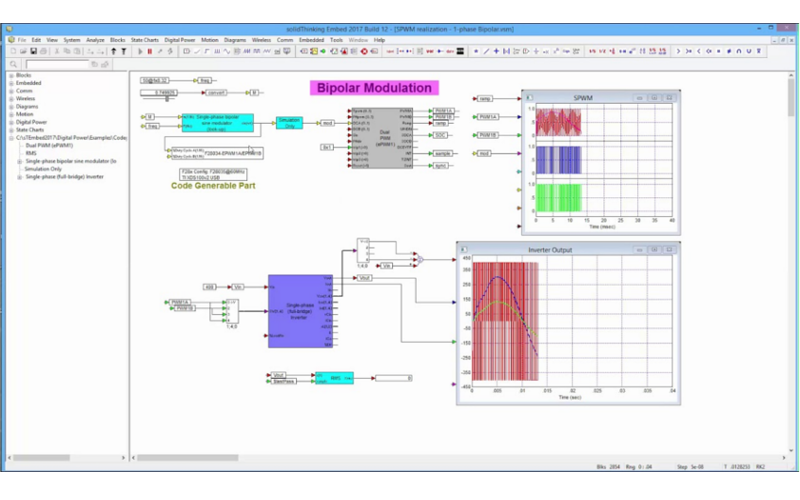
\includegraphics[width=0.9\linewidth]{Figures/lang-vissim}
               \caption{\label{tab:VisSim}VisSim}
               \strut
               \end{subfigure}
                &
               \begin{subfigure}{0.35\linewidth}\centering
               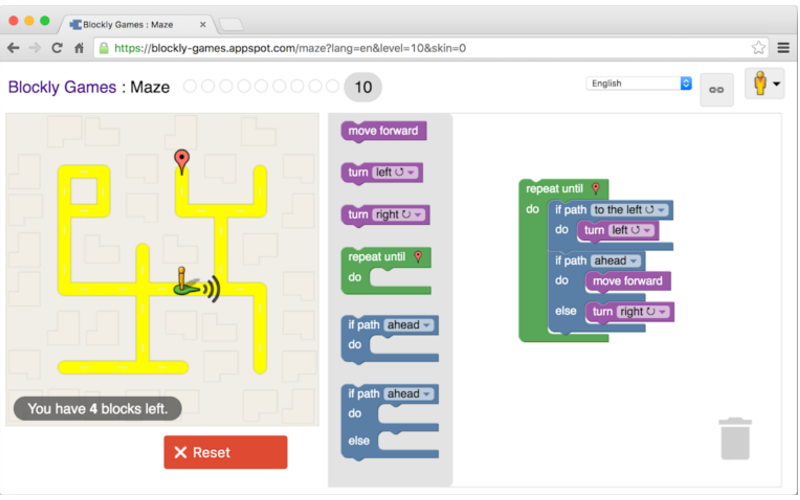
\includegraphics[width=0.9\linewidth]{Figures/lang-blockly}
               \caption{\label{tab:Blockly}blockly}
               \strut
               \end{subfigure}
                \\ \hline
               \begin{subfigure}{0.35\linewidth}\centering
               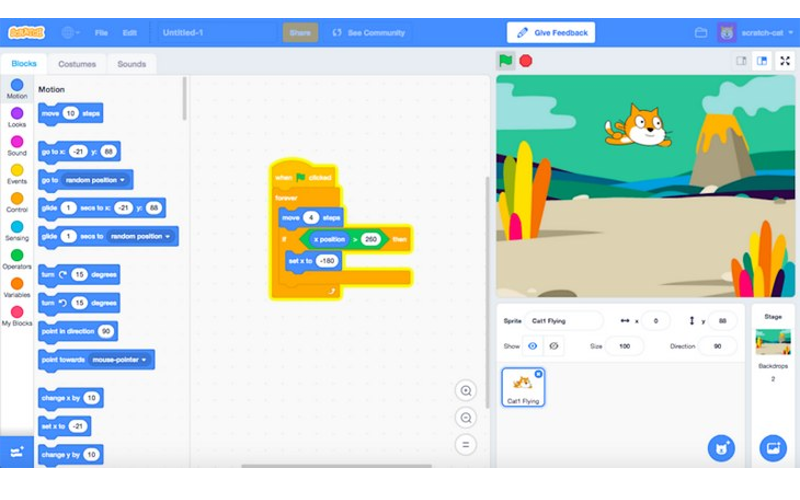
\includegraphics[width=0.9\linewidth]{Figures/lang-Scratch}
               \caption{\label{tab:Scratch}Scratch}
               \strut
               \end{subfigure}
                &
               \begin{subfigure}{0.35\linewidth}\centering
               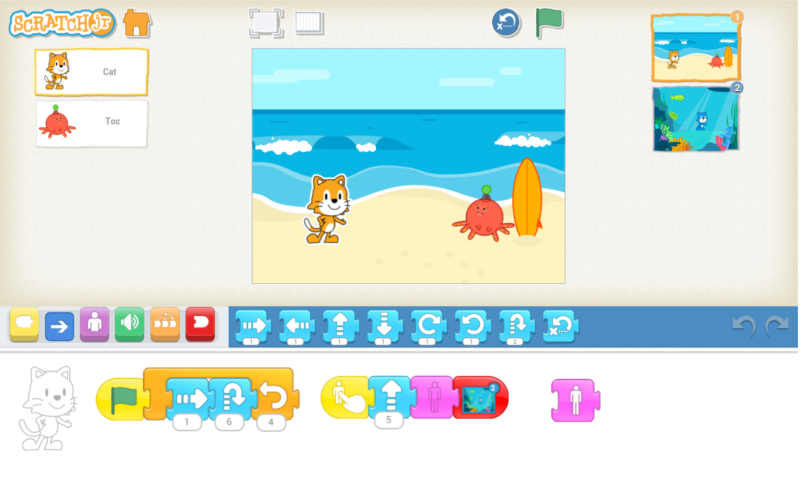
\includegraphics[width=0.9\linewidth]{Figures/lang-JrScratch}
               \caption{\label{tab:ScratchJr}ScratchJr}
               \strut
               \end{subfigure}
                \\ \hline
               \begin{subfigure}{0.35\linewidth}\centering
               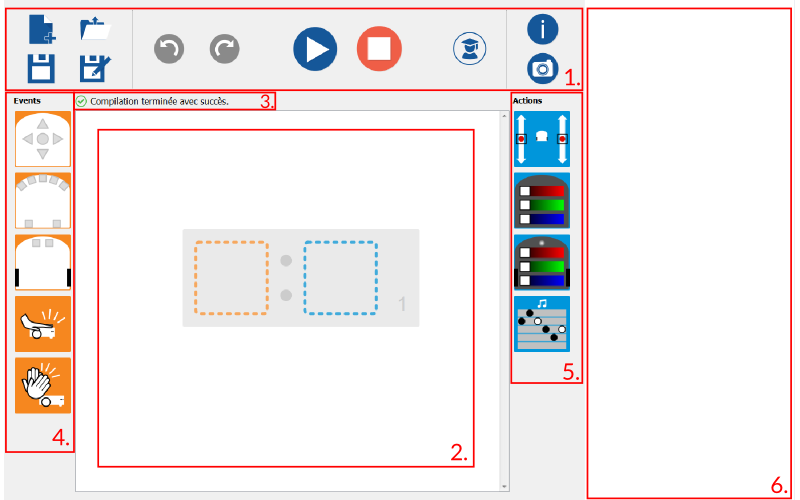
\includegraphics[width=0.9\linewidth]{Figures/lang-vpl2}
               \caption{\label{tab:VPL}Aseba-VPL}
               \strut
               \end{subfigure}
                &
               \begin{subfigure}{0.35\linewidth}\centering
               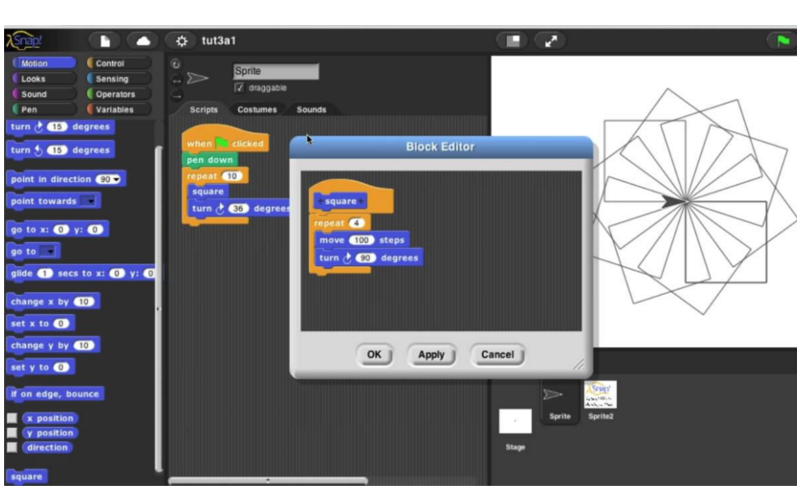
\includegraphics[width=0.9\linewidth]{Figures/lang-snap}
               \caption{\label{tab:Snap}\textit{Snap!} Blocks}
               \strut
               \end{subfigure}
                \\ \hline
            \end{tabular}
            \caption{Langage de programmation visuel}\label{tab:langue}
            \end{table}
            \paragraph{VisSim}\citeT{tab:VisSim}
                Sa première implémentation en 1989, fait de ce langage l'un des tout premiers langages visuels.
                Il permet de modéliser et de simuler des systèmes dynamiques complexes. Son interface permet de manipuler par glisser/déposer des blocs de diagrammes à assembler pour constituer un programme. Il est largement utilisé dans le domaine des systèmes de contrôle et de traitement numérique de signal. Il intègre des blocs pour l’arithmétique, le booléen et les fonctions transcendantes, ainsi que des filtres numériques, des fonctions de transfert, l’intégration numérique et un interactif de traçage.
            \paragraph{VPL}\label{sec:VPL}
                \glsdesc{vpl}~\citeT{tab:VPL}est un langage de programmation développé dans le cadre du projet Thymio et est spécifique à ce robot.
                Dans VPL, un programme est écrit en assemblant des paires de blocs d'événements et d'actions. La fenêtre se présente ainsi:
                \begin{enumerate}\myItemStyle
                    \item La barre d'outils contient les boutons classiques de gestion.
                    \item Cette zone est dédiée à la construction du programme.
                    \item Cette ligne indique si les paires événement-action composant le programme sont correctes et complètes, le cas échéant, elle retourne l'erreur.
                    \item Les blocs d'événements déterminent quand le robot doit démarrer une action. Ces blocs peuvent être ajoutés au programme en cliquant dessus ou en les glissant sur le carré gauche d'une paire événement-action qui apparaît dans la zone programme.
                    \item Les blocs d'action déterminent comment le robot doit réagir. Ces blocs s'ajoutent comme les blocs événement.
                    \item En mode indépendant de Studio, le programme texte correspondant au programme graphique est écrit dans cette zone.
                \end{enumerate}{}
                Ce langage est accessible pour de très jeunes utilisateurs ( \eg ne sachant ni lire ni écrire).
            \paragraph{Blockly}\label{sec:Blockly}
                \glsdesc{bloc}~\citeT{tab:Blockly}est une bibliothèque logicielle JavaScript permettant de créer des environnements de développement utilisant un langage graphique. Présenté à la Maker Faire 2012, c'est un projet open source de Google, publié sous la licence Apache 2.01.
                Concrètement, il s'agit d'assembler des blocs dans un éditeur visuel directement sur une page web. Pour cela l'interface de Blockly propose deux éléments: \textit{1.} une boîte à outils contenant l'ensemble des blocs disponibles pour créer le programme (présentés seuls ou en catégories); \textit{2.} un espace de travail. Les blocs doivent être déplacés (par \cro{glisser-déposer}) au sein de l'espace de travail afin de créer un programme. En plus des blocs de base, Blockly fournit un outil appelé Blockly Developer Tools pour créer de nouveaux blocs. 
                Comme avec Scratch, le code généré est exempt d'erreurs de syntaxe. Cependant, à la différence de Scratch qui nécessite Flash, Blockly n'utilise pas de logiciels propriétaires. De plus, le code produit peut être exporté en JavaScript, Python, PHP, Dart ou Lua.\par%
            \myPhantom{paragraph}{Scrtach}\label{sec:Scrtach}
                \subparagraph{\texorpdfstring{\indent Scratch}{Scratch}}
                    \glsdesc{scra}~\citeT{tab:Scratch}offre la possibilité de programmer des histoires interactives, des jeux, des animations - et de partager ces créations avec d'autres dans une communauté en ligne.
                    Depuis janvier 2019 scratch3 est utilisable directement en ligne; sa version antérieur 1.x nécessitait, elle, une installation et sa version 2.x, bien que exécutable en ligne, nécessitait AdobeFlash (ou AdobeAir) car elle était rédigée en ActionScript (un dérivé de JavaScript).
                    Le code du logiciel Scratch est publié, jusqu’à la version 1.3, sous la Licence \textit{Scratch Source Code} (libre à l’exception du logo, de la marque et du système de téléversement sur le site web officiel).
                    La version 1.4 ainsi que les versions de la branche 2.x sont publiées sous la licence libre GPL afin de permettre une diffusion plus large du logiciel, et notamment dans les distributions Linux. Cependant, la seconde génération écrite en ActionScript nécessite un moteur d’exécution Flash propriétaire et n’est donc pas incluse dans les dépôts de distributions telles que Debian.
                    Le code de la troisième version, désormais écrite en JavaScript est disponible en licence BSD-3-clauses (à l’exception de Scratch-blocks, publié sous la licence Apache 2.0, libre également); elle propose également un Editeur Off-line accessible sur le site du MIT Media Lab. 
                    C'est le langage le plus largement utilisé au collège car avec la réforme des collèges en France de 2015~\citeS{sec:programme-officiel} apparaissent les notions de codage et de programmation et donc des exercices (illustrés en Scratch) au Brevet.
                    Ce logiciel est traduit en soixante-dix langues et le site web comptait plus de 45 millions d'utilisateurs en septembre 2019, et plus de 43 millions de projets partagés.
                \subparagraph{\texorpdfstring{\indent ScratchJr}{ScratchJr}}\label{sec:ScrtachJr}
                    C'est un langage de programmation visuel~\citeT{tab:ScratchJr}également conçu par \textit{MIT Media Lab} pour introduire les compétences de codage aux enfants âgés de 5 à 7 ans. %En créant des projets dans ScratchJr, les jeunes enfants peuvent apprendre à penser de manière créative et à raisonner de manière systématique, même s'ils ne savent pas lire. 
                    Il est disponible sous forme d'application gratuite pour iOS, Android et Chromebook.
                    ScratchJr est un dérivé du langage Scratch. Le codage dans Scratch nécessite des compétences de base en lecture, parfois pas encore acquise chez certains individus. Par conséquent, les créateurs ont perçu le besoin d’une autre langue qui fournirait un moyen simplifié d’apprendre à coder notamment pour les plus jeunes.
                    Les enfants créent du code sous forme de blocs \tiret{entièrement basés sur des icônes (pas de texte)} et manipulent des sprites (qui peuvent être des personnages ou des objets). ScratchJr est livré avec une bibliothèque de sprites, qui peuvent être modifiés ou créés à l’aide de \cro{l'éditeur de peinture}.
                    Les blocs sont connectés de gauche à droite, comme les mots d'une pĥrase.
                    L'interface utilisateur est beaucoup plus simple que celle de Scratch. Le nombre de catégories et le nombre de blocs dans chaque catégorie ont été réduits, de sorte que seuls les plus élémentaires ont été conservés.\par%
                    Vassilis Komis~\citeB{komis2017analyse} présente une analyse d’ordre cognitif et didactique de l’environnement de programmation ScratchJr. Il s’inscrit dans une approche d’apprentissage de concepts de base de programmation et de développement des compétences associées. Néanmoins, malgré ce que son aspect visuel et son ergonomie syntaxique laissent sous-entendre, l'analyse montre que la sémantique du ScratchJr n’est ni simple ni toujours intuitive. Par conséquent, ils souligne qu' \gui{un enseignement approprié du ScratchJr, sous une problématique gérée par les apports de la didactique de l’informatique s’avère nécessaire si on veut en tirer des profits cognitifs pendant son apprentissage}. Or, l'avancée des recherches concernant l’apprentissage de la programmation pendant la petite enfance (à l’aide des environnements visuels de programmation) n’étant qu’à ses débuts, plusieurs questions restent ouvertes sur la pertinence de tel outil, notamment dans le cas de mésusage.
            \paragraph{Snap}\label{sec:Snap}
                La force de \sht{snap}~\citeT{tab:Snap} est qu'il a su garder la puissance d'expression qu'a un langage de programmation classique pour représenter et résoudre des objets complexes, et ceci tout en alliant un style graphique ne nécessitant pas de bagage particulier pour le manipuler. Les procédures, autrement dit les blocs, possèdent un code forme et couleur rendant son utilisation plus intuitive et attractive. Il est utilisable directement en ligne~\citeURL{snap} et dispose d'un didacticiel~\citeB{garcia2015beauty} permettant une prise en main rapide et ludique du langage. Bien que très similaire dans la forme à Scratch, il possède de nombreuses différences de fond~\citeS{sec:snap_choice}.
        \subsubsection{Multilingues}
            \paragraph{API web}\label{sec:API}
                Dans le cas de Poppy, le contrôle du robot se fait en python via la bibliothèque dédiée: pypot (disponible sur github). Les Poppy sont donc nativement contrôlables en python. Mais une des forces de la plateforme et d'offrir une \sht{api}
                \begin{figure}[!h]
                \begin{minipage}{0.525\linewidth}
                    \centering
                    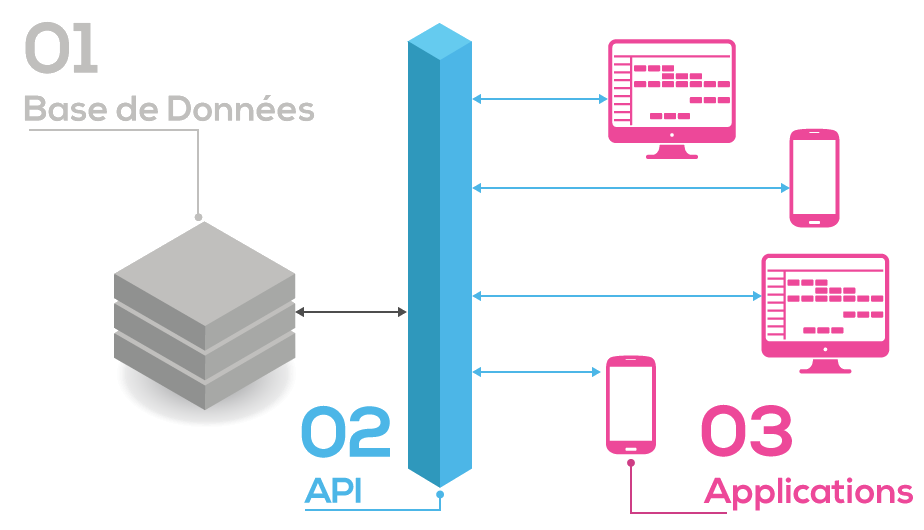
\includegraphics[width=0.9\linewidth]{Figures/Open_classroom-api}
                    \caption{Architecture générale d'une API}\label{fig:API}
                \end{minipage}
                \hfill
                \begin{minipage}{0.445\linewidth}
                \myDefautStyle
                     Elle permet, via un serveur web local, d'interpréter des requêtes HTTP en instruction python. Ainsi, tout langage de programmation intégrant l'envoi de requêtes web peut potentiellement être utilisé pour contrôler le robot.
                     \\
                \end{minipage}
                \end{figure}\par%
                Plus généralement, une \glsdesc{api} est une façade qui délimite l'espace par laquelle un logiciel offre des services à d'autres logiciels. Ainsi, l'objectif est de fournir une porte d'accès à une fonctionnalité en cachant les détails de sa mise en œuvre. Elle peut comporter des classes, des méthodes ou des fonctions, des types de données et des constantes qui lui sont propres. Le plus souvent, elle fournit une solution à un problème informatique en faisant abstraction de son fonctionnement.
    \subsection{Des exemples}\label{sec:bot}
        \begin{table}[!h]
            \centering
            \begin{tabular}{|c|c|c|c|}
            \hline
                \begin{subtable}{0.215\linewidth}
                    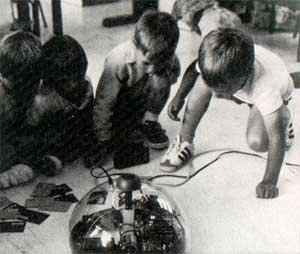
\includegraphics[width=\linewidth]{Figures/bot-logo.jpg}
                    \subcaption{Tortue Logo}\label{tab:Logo}
                \end{subtable}
                 &
                \begin{subtable}{0.215\linewidth}
                    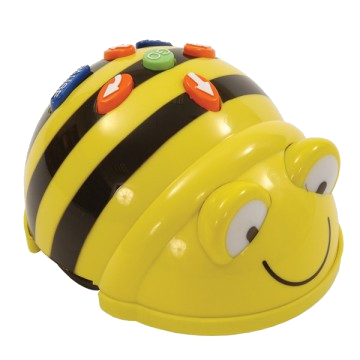
\includegraphics[width=\linewidth]{Figures/bot-beebot.png}
                    \subcaption{BeeBot}\label{tab:BeeBot}
                \end{subtable}
                 &
                \begin{subtable}{0.215\linewidth}
                    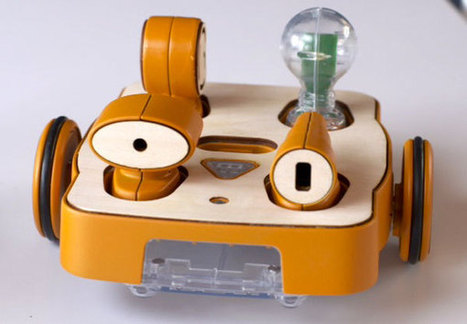
\includegraphics[width=\linewidth]{Figures/bot-kibo.jpeg}
                    \subcaption{Kibo}\label{tab:Kibo}
                \end{subtable}
                 &
                \begin{subtable}{0.215\linewidth}
                    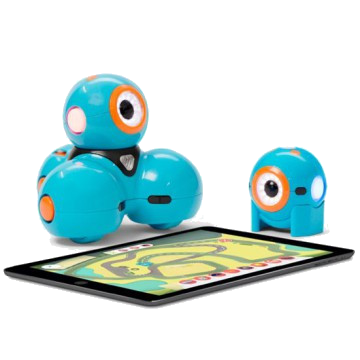
\includegraphics[width=\linewidth]{Figures/bot-dashdot.png}
                    \subcaption{Dash \& Dot}\vspace{0.2cm}\label{tab:DashDot}
                \end{subtable}
                 \\ \hline
                \begin{subtable}{0.215\linewidth}
                    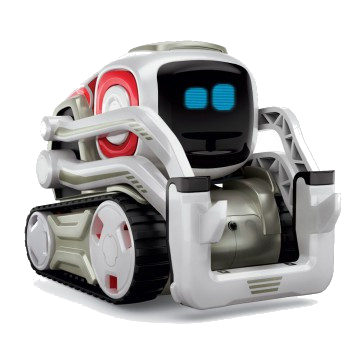
\includegraphics[width=\linewidth]{Figures/bot-cozmo.png}
                    \subcaption{Cozmo}\label{tab:Cozmo}
                \end{subtable}
                 &
                \begin{subtable}{0.215\linewidth}
                    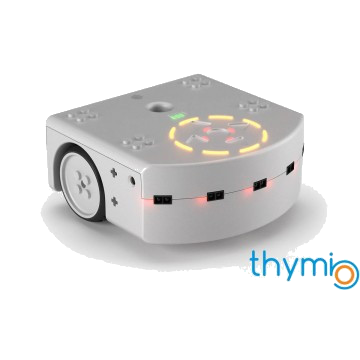
\includegraphics[width=\linewidth]{Figures/bot-thymio.png}
                    \subcaption{Thymio}\label{tab:Thymio}
                \end{subtable}
                 &
                \begin{subtable}{0.215\linewidth}
                    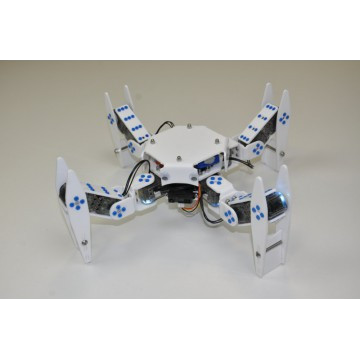
\includegraphics[width=\linewidth]{Figures/bot-metabot.png}
                    \subcaption{Metabot}\label{tab:Metabot}
                \end{subtable}
                 &
                \begin{subtable}{0.215\linewidth}
                    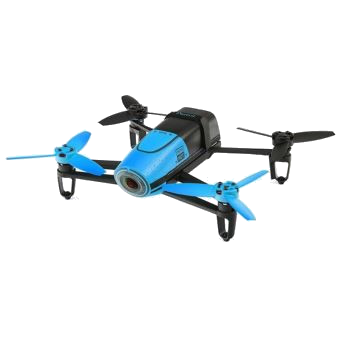
\includegraphics[width=\linewidth]{Figures/bot-bebop.png}
                    \subcaption{Bebop}\vspace{0.2cm}\label{tab:Bebop}
                \end{subtable}
                 \\ \hline
                \begin{subtable}{0.215\linewidth}
                    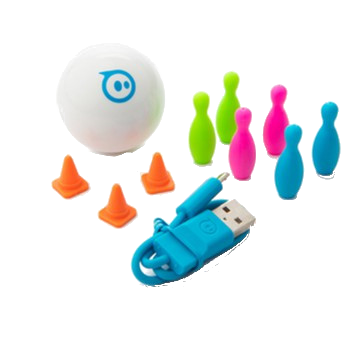
\includegraphics[width=\linewidth]{Figures/bot-sphero.png}
                    \subcaption{sphero}\label{tab:Sphero}
                \end{subtable}
                 &
                \begin{subtable}{0.215\linewidth}
                    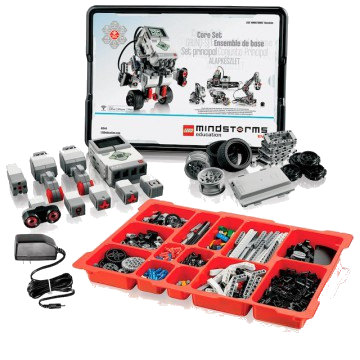
\includegraphics[width=\linewidth]{Figures/bot-mindstorm.png}
                    \subcaption{Mindstorm}\label{tab:Mindstorm}
                \end{subtable}
                 &
                \begin{subtable}{0.215\linewidth}
                    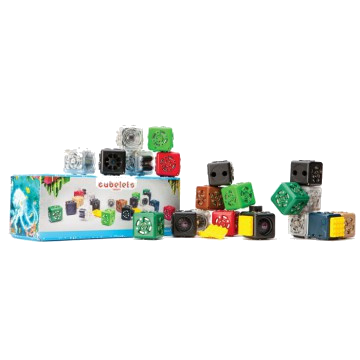
\includegraphics[width=\linewidth]{Figures/bot-cubelets.png}
                    \subcaption{Cubelets}\label{tab:Cubelets}
                \end{subtable}
                 &
                \begin{subtable}{0.215\linewidth}
                    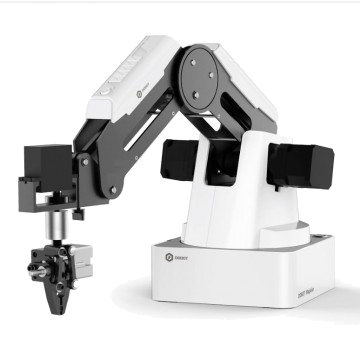
\includegraphics[width=\linewidth]{Figures/bot-Dobot.png}
                    \subcaption{Dobot}\vspace{0.2cm}\label{tab:Dobot}
                \end{subtable}
                 \\ \hline
                \begin{subtable}{0.215\linewidth}
                    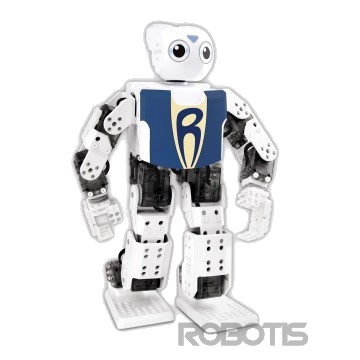
\includegraphics[width=\linewidth]{Figures/bot-darwin.png}
                    \subcaption{Darwin}\label{tab:Darwin}
                \end{subtable}
                 &
                \begin{subtable}{0.215\linewidth}
                    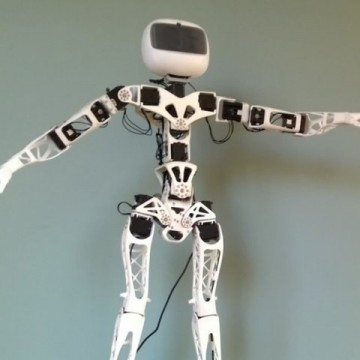
\includegraphics[width=.9\linewidth]{Figures/bot-poppy.jpg}
                    \subcaption{Poppy-Huma}\label{tab:Poppy}
                \end{subtable}
                 &
                \begin{subtable}{0.215\linewidth}
                    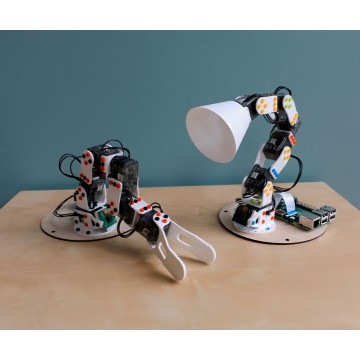
\includegraphics[width=.9\linewidth]{Figures/bot-ergo.png}
                    \subcaption{Poppy-ErgoJr}\label{tab:Ergo}
                \end{subtable}
                 &
                \begin{subtable}{0.215\linewidth}
                    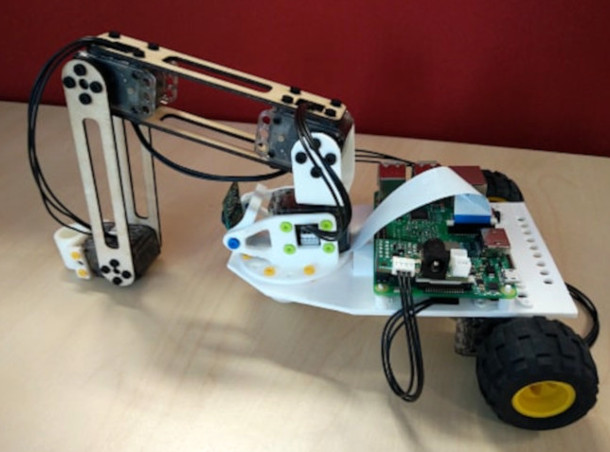
\includegraphics[width=\linewidth]{Figures/Poppy-dragster.jpg}
                    \subcaption{Poppy-Dragster}\vspace{0.2cm}\label{tab:Dragster}
                \end{subtable}
                 \\ \hline
            \end{tabular}
            \caption{Trombinoscope robotique}
            \label{tab:bot}
        \end{table}\par%
        \begin{comment}
        \begin{table}[!h]
            \centering
            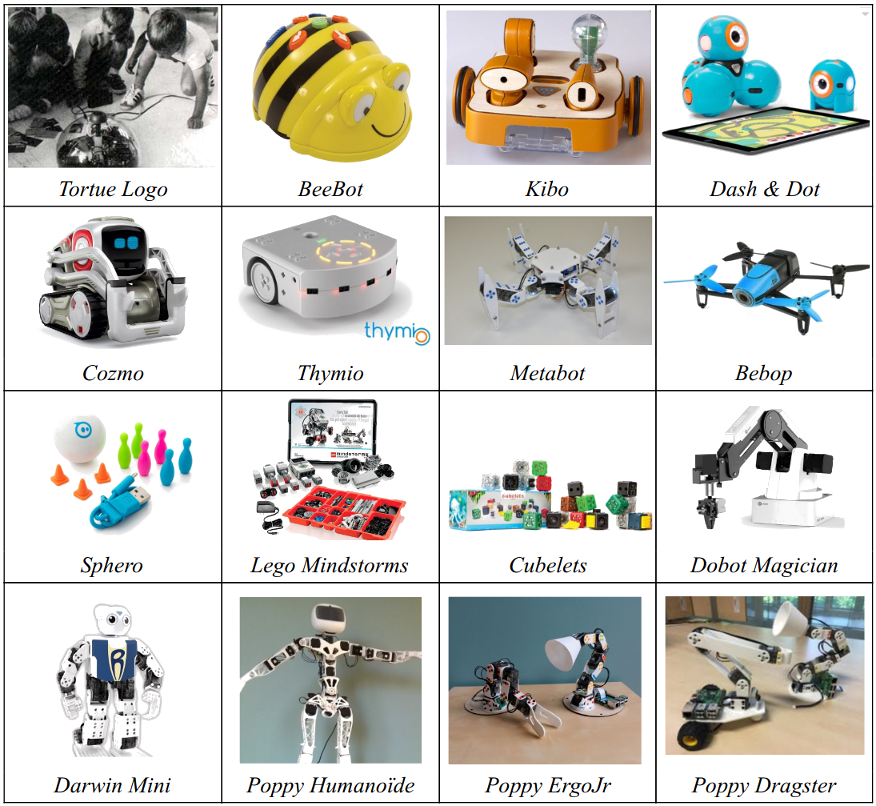
\includegraphics[width=0.9\linewidth]{Figures/bot-trombi}
            \caption{Trombinoscope robotique}\label{tab:bot}
        \end{table}
        \end{comment}
        \paragraph{Beebot et Kibo}\label{sec:BeeBot}
            Disponible pour les enseignants sous forme de pack de 6 robots, Bee-Bot~\citeT{tab:BeeBot} rappelle les formes de la Tortue Logo~\citeT{tab:Logo}
            Bee-Bot offre une multitude de possibilités d'enseignement. Plusieurs tapis et cartes d'activités permettent de mettre en place des ateliers clés en main ou bien personnalisés. 
            En robot de maternelle, Bee-Bot~\citeT{tab:BeeBot} vous permet ainsi d'améliorer les capacités des élèves à se repérer dans l'espace et à utiliser le bon vocabulaire pour déplacer le robot. Il permet également de mettre en place des groupes d'apprentissage autour de l'alphabet ou des premières opérations mathématiques.
            En robot pour la primaire, Bee-Bot se présentera plus comme un \textit{add-on}, un \textit{goodies} dans d'autres activités comme la géographie, les règles de la grammaire et de l'orthographe, ou de calculs de plus en plus complexes, mais ces capacités restent limitées. Dans les activités d'apprentissage des concepts préliminaires de programmation, sa pertinence dépendra de l'usage effectif du robot par l'enseignant et du cadre pédagogique et scénaristique qu'il y développera~\citeB{komis2011robotique}.\par%
            Développé par la firme KinderLab Robotics, Kibo~\citeT{tab:Kibo} est un robot à assembler soi-même grâce à des composants modulaires. Il ne requiert pas l’utilisation d’un appareil numérique dans sa réalisation, il favorise l'esprit créatif et le travail manuel. 
            Il est orienté davantage pour les quatre à sept ans,  qui pour le construire se servent d’un module à deux roues muni d’un moteur comme unité de base. A ceci s’ajoute des blocs de bois colorés comportants des indications et des codes barres pour faciliter la programmation. Après avoir personnalisé son robot, il peut lui attribuer une fonction spécifique suivant la demande. Il suffit ensuite d’appuyer sur un bouton pour lancer le programme et animer le robot.
            L'objectif est de laisser libre cours à l'imagination en matière de création, puis in-finé durant la programmation.  Plusieurs phases de test, parfois à grand échelle, ont déjà été réalisées~\citeB{sullivan2015kibo,sullivan2017imagining}. Cependant il n'est toujours pas disponible commercialement.
        \paragraph{Dash\&dot}\label{sec:DashDot}
            Ce sont 2 robots~\citeT{tab:DashDot} programmables et interactifs conçus par Make Wonderest. Dash est présenté comme l’aventurier. Grâce à sa tête rotative et ses trois roues, il se déplace facilement. Il peut détecter des objets et des obstacles et réaliser des actions en conséquence. il dispose de différents accessoires lui permettant de ramasser, soulever, dessiner ou jouer de la musique. Dot, présenté comme le compagnon, est entièrement rond, il détecte à quel moment il est attrapé, soulevé ou bougé. Il peut également transmettre des informations ou  des ordres à Dash. Les 2 compagnons sont programmables par le biais de l’appli Go (téléchargable avec iOS ou Android), et avec le langage visuel Blockly ou Scratch. 
            Ces robots offrent donc de nombreuses possibilités tant en terme d'interaction, qu'en terme de programmation ou de pédagogie. Cependant, il n'est pas directement modifiable, bien qu'il intègre des fixations pour cube \textit{lego}, son usage reste relativement contraint au développement effectué par la société mère. 
        \paragraph{Cozmo}\label{sec:Cozmo}\nocite{kusumota2018open} 
            Ce petit robot~\citeT{tab:Cozmo} mise essentiellement sur le côté expressif, via ses yeux, ses bruits et ses déplacements, il produit un comportement, \cro{une personnalité}  comparable à un personnage de cartoon. Pour réaliser cela, Anki, la société créatrice de Cozmo, a équipé ce robot de nombreux capteurs lui permettant, entre autres, de reconnaître les visages et d'adapter ses réactions en conséquence, mais il peut également apprendre une infinité de nouvelles activités. Il apprend également à apprivoiser son environnement, et prend des décisions qui peuvent varier selon \cro{son humeur}. Plusieurs petits jeux sont directement implémentés, notamment avec l'appui des 3 cubes lumineux qui l'accompagnent.
            Via son application CodeLab compatible iOS et Android, 2 interfaces de programmation visuelle basée sur Scratch sont disponibles:
            \textit{1.} Le mode Sandbox qui permet d'appréhender les fonctionnalités du robot: assembler des blocs d'action, d'émotion ou de réaction dans l'ordre souhaité pour définir un comportement; \textit{2.} le mode constructeur qui permet d'accéder aux fonctions supérieures de Cozmo. Pour les utilisateurs avancés, Cozmo est programmable sur Python et dispose également d'un SDK dédié. Il peut également faire office de hub central pour objets connectés, allant jusqu'à apprendre à contrôler les lumières d'une smart-home ou interagir avec l’assistant personnel intelligent Google Home.
            Mais bien qu'il semble offrir de grandes capacités, d'un point de vue pédagogique, au contraire de Thymio, ce robot ne cherche pas à rendre explicite les principes sous-jacents à son fonctionnement. Typiquement, la majorité des capteurs son dissimulés. De plus, l'illusion de la personnalité qu'il génére \tiret{plutôt réaliste} donne un faux-semblant d'être vivant et d'intelligence; rendant l'amalgame facile.
        \paragraph{Thymio}\label{sec:thymio}
            C'est un robot~\citeT{tab:Thymio} développé en collaboration par l’École Polytechnique Fédérale de Lausanne (EPFL) et l'École Cantonale d'Art de Lausanne (écal). Leur but est de fournir un robot pédagogique à bas coût~\citeB{riedo2013thymio, mondada2017bringing}. Thymio est totalement open source, que ce soit au niveau logiciel ou matériel.
            Thymio possède de nombreux capteurs facilement identifiables, notamment ses capteurs d'infrarouges qui lui permet d'éviter les obstacles ou de suivre une ligne (noir) au sol.
            %(microphone, récepteur infrarouge, température, proximité, accéléromètre 3 axes, capteurs au sol pour le suivi de lignes), actionneurs (moteurs, haut-parleurs, LEDs), connecteurs (USB, carte mémoire) et bien sûr, le fameux module WiFi ! 
            Il possède également un emplacement spécialement conçu pour y mettre un crayon et utiliser le robot pour dessiner, ainsi que des fixations mécaniques compatibles Lego.
            Un feedback en temps réel sur les différentes parties du code en train d’être exécutées par le robot, ainsi que le retour des données provenant des différents capteurs et moteurs est fourni via l'interface Aseba~\citeS{sec:Aseba} et VPL~\citeS{sec:VPL}.
            Au démarrage, Thymio possède 6 comportements de démonstration:
            \begin{enumerate}\myItemStyle
            \small
                \item L'amical (vert): Thymio suit un objet en face de lui.
                \item L'explorateur (jaune): explore l'environnement, tout en évitant les obstacles.
                \item Le peureux (rouge): détecte les chocs, la chute libre et montre la direction de la gravité.
                \item L'enquêteur (turquoise): suit une piste (ligne noire sur le sol).
                \item L'obéissant (mauve): suit les ordres donnés par les boutons ou une télécommande.
                \item L'attentif (bleu): réagit au son. On peut le commander avec des clappements de mains: 1 clap = tourne ou avance tout droit; 2 claps = marche / arrêt; 3 claps = fait un cercle.
            \end{enumerate}{}\par%
            Ce robot possède une communauté en pleine expansion~\citeURL{thymio_forum}. Plusieurs projets d'envergure internationale existent notamment autour de l'éducation comme pour le projet: R2T2 (Remote Rescue Thymio II)~\citeURL{thymio_r2t2}. De plus en plus d'établissements scolaires (maternelle - primaire - collège) s'équipent de ce robot qui offre un excellent rapport possibilité / prix. Côté grand public il reste encore peu diffusé, notamment de part son absence dans les grandes surfaces ou les magasins de jouets: il se trouve dans des magasins spécialisés en robotique \etou en éducation tel que Génération Robot~\citeURL{GR}.
        \paragraph{Bebop}\label{sec:Bebop}\nocite{krajnik2011ar}
            C'est un robot drone~\citeT{tab:Bebop} développé par la société Parrot. Il peut voler, filmer et photographier en intérieur comme en extérieur. Ce robot n'offre pas de fonctionnalité ou de performance particulièrement dédiée à des visions éducatives. En revanche, Parrot dispose d'un service spécifique: Parrot Education qui collabore en effet avec Tynker, MathWorks, Swift Playground, Blockly et plusieurs autres organisations à vocation éducative, pour aider les professeurs à créer, partager et adapter leurs projets à leurs programmes d’enseignement.
        \paragraph{Meta-bot}\label{sec:Metabot}
            Metabot est robot quadrupède~\citeT{tab:Metabot}fruit d’un partenariat entre la start-up Rhoban System S.A.S, le LaBRI (Laboratoire bordelais de recherche en informatique), l’association Robot Campus ainsi que Bordeaux INP et le cluster Aquitaine Robotics.
            La plateforme Metabot s’appuie sur des composants standards (moteurs, électronique, batterie, \etc) et sur des pièces imprimables en 3D. Cette plateforme s’adresse autant aux passionnés qu’aux enseignants et chercheurs~\citeB{passault2016metabot}. Un des objectifs de Metabot est de fédérer une communauté autour des robots à pattes, c’est pourquoi les pièces et le logiciel sont entièrement disponibles en open-source. Il est disponible sous forme de kit qui requiert un assemblage, et permet la modification. Ce robot est doté de 12 servomoteurs, d’une centrale inertielle 9 axes et d’un capteur de distance frontal. Il est contrôlé par un microprocesseur ARM (STM32F103 @72Mhz). Les pièces de la structure peuvent être fabriquées à l’aide d’une imprimante 3D ou d’une découpeuse laser.
            Il posséde un simulateur en ligne~\citeURL{metabot_simu} et il est programmable via un un environnement graphique: Metabot Blocks (\textit{Sctrach like}).